%\begin{abstract}
%When people seek to understand concepts from an incomplete set of examples and counterexamples, there is usually an exponentially large number of classification rules that can correctly classify the observed data, depending which features of the examples are used to construct these rules.
%A mechanistic approximation of human concept-learning should help to explain how humans preferentially fixate on certain sets of features to construct classification rules, even when many others could also be used to correctly classify the same observed data. Here, we exploit the tools of propositional logic to develop an experimental framework that controls the minimal rules that are \textit{simultaneously} consistent with the presented examples.
% For example, our framework allows us to present participants with concepts consistent with a disjunction \textit{and also} with a conjunction, depending on which features are used to build the rule. Similarly, it allows us to present concepts that are simultaneously consistent with two or more rules of different complexity and using different features.
% Importantly, our framework fully controls which minimal rules compete to explain the examples, guaranteeing that any potential rule built over a tertiary set of features will be inconsistent with the observed examples. Then, without relying on supplementary attention-tracking mechanisms (e.g.\ eye-tracking), we recover the features used by the participant to build the classification rule. We exploit our framework in an experiment with a sequence of such competitive trials, illustrating the emergence of various transfer effects that bias participants' prior attention to specific sets of features during learning.
%\end{abstract}

%OJO QUE NO ESTÁ ACTUALIZADO

\chapter{BORRAR: A logical framework to study concept-learning biases in the presence of multiple explanations}

%%%%%%%%%%%%%%%%%%%%%%%% INTRO %%%%%%%%%%%%%%%%%%%%%%%%%%%%

% \section{Introduction}\label{Section:Introduction}


% \widesergio{Apuntar a Behavior Research Methods para octubre  https://www.springer.com/journal/13428 

% Segunda opción:  Memory and Cognition https://www.springer.com/journal/13421}
% \widesergio{    
% Santi: Poner referencias que nos recomendaron. Revisar la estructura general según BRM?  Reenfocar intro, abstract.\\
% Pablo: Tener disponibles datos experimentales y el setup preciso de cada trial. Incluir en la intro la estrategia del diseno experimental: si el participante describe el concepto usando un conjunto de variables que no contengan a las variables de interes, los mismos valores quedan como dentro y como fuera del concepto. Actualizar histograma para variables en vez de scores. Generar lista de datos.\\
% Sergio:  Apéndice E con Teorema que fundamenta lo que hacemos. Revisión general de setup experimental; separación de conceptos visibles vs escondidos. Revisión general de notación. Por lo que veo, siempre mostramos toda la interseccion y todo el complemento de la union, ver en Dropbox Elementos mostrados en los trials.txt)
% }

% \widesanti{En BRM dice

% The following are examples of appropriate Open Practices Statements:

% The data and materials for all experiments are available at (url for the site hosting the data and materials) and Experiment 1 was preregistered (url for the preregistration).

% Es bueno, porque habla de preregistración. También deberíamos poner los datos en algun lugar. %Sergio: Hay que anonimizar los Turker ID? % Estaría bueno poner también los datos del experimento mismo: el universo mostrado y lo mostrado en la generalización. Idealmente con notas para que no sea tan abstruso tener listas de listas de ceros y unos.
% }


%Regardless of whether human cognitive processes can be better explained with similarity-based or with rule-based accounts \cite{hahn1998similarity}, 
Concept acquisition is a key and widely studied aspect of human daily cognition \cite{cohen2005handbook, ashby2011human}. Many researchers have claimed that a coding system and a set of rules underlie some of our  abilities to acquire concepts \cite{nosofsky1994rule,tenenbaum2011grow,maddox1993comparing}, and it has been observed that we seem to learn concepts of objects with more ease when there are `simpler' rules that can explain those groupings \cite{shepard1961learning, nosofsky1994comparing, rehder2005eyetracking, lewandowsky2011working,feldman2000minimization,blair2003easy,minda2001prototypes}. 
% This is even true in finite and small domains where some kind of `pure memorization' would seem to be a valid strategy \cite{blair2003easy,minda2001prototypes}.

In the real-world, humans learn concept descriptions while simultaneously deciding on which features to attend \cite{schyns1998development}; and the selected set of features usually determines the structure and complexity of the minimal rules that can describe the concept. For example, the concept \textit{dog} can be explained as {\em a four-legged pet that is not a cat} or as {\em an animal for hunting, herding, pulling sledges or company}. Both descriptions are fully compatible with the concept \textit{dog}, but our experience induces us to choose different relevant features to define the concept. While the first description of {\em dog} could be very well be given by a child having a dog at home, the second could be given by a shepherd or perhaps an ethologist. It is likely that the features used to describe {\em dog} by each agent allows them to compactly describe the concept, while simultaneously separating it from other concepts frequently encountered in their environment. Here, we ask about which features participants use to describe concepts, depending on the logical structure of the description using those features and also on their exposure to previous concepts. Why will someone use {\em cat} or {\em hunting} to define {\em dog}?

\begin{figure}
\begin{center}
	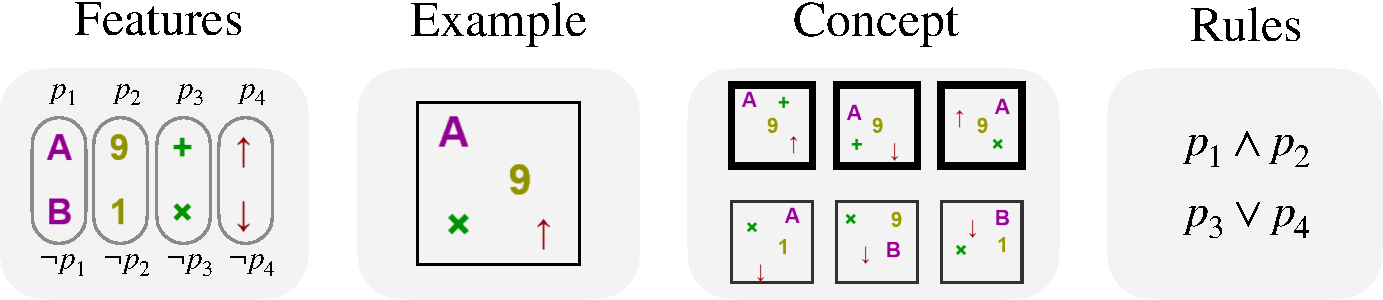
\includegraphics[scale=.6]{intro_notation.pdf}
\end{center}\caption{Illustration of the features $\{p_1,p_2,p_3,p_4\}$, the example $(1,1,0,1)$, and a concept (positive example are marked with bold boundaries and negative examples with thin boundaries). The concept can be explained with the two minimal rules $p_1 \land p_2$ or $p_3 \lor p_4$, depending on which features are used to build the rule.}
\label{fig:intro_notation}
\end{figure}
%\sergio{En el caption de la figura decía Example $(1,1,0,0)$. Lo corregí a $(1,1,0,1)$}\santi{Muy buena esta explicación! Claro, bien, Sergio. Habría que cambiarlo en el texto también. no? }


In propositional concept-learning experiments, participants are presented with a set of \textit{examples}, each conformed of $N$ propositional \textit{features}, which can take positive or negative values. For instance, for $N=4$ one example can be logically represented as the element $(1,1,0,1)$, which takes positive values for the first, second and fourth features and negative for the second one, as illustrated in Fig. \ref{fig:intro_notation}. A \textit{concept} can be intuitively understood as a set of examples, some of them marked as belonging to the concept and the rest marked as not belonging, i.e.\ positive and negative examples. In Fig. \ref{fig:intro_notation} we show an example of an \textit{underdetermined} concept, in the sense that, since the entire universe of examples is not shown (i.e. the $2^4$ examples), different determined concepts can be consistent with this smaller set when extending the set of examples to the full universe. %\sergio{Duda: en los experimentos típicos estos se muestran ejemplos negativos, no?}.
A \textit{rule} consistent with the concept is a logical formula built with the features and the conjunction ($\land$), disjunction ($\lor$) and negation ($\lnot$) operators, which evaluates to true for objects belonging to the concept and false otherwise (e.g. $p_1 \land p_2$, where $p_i$ is the $i^{th}$ feature, see Fig. 
\ref{fig:intro_notation}). The \textit{minimal description length} (\textit{MDL}) of a concept is the length of the shortest rule consistent with the concept \cite{grunwald2007minimum}. Importantly, most studies of subjective difficulty with concept-learning are designed such that a {\em single} minimal rule can be used to describe the concept (e.g. $p_1 \land p_2$) \cite{ashby2005human,feldman2000minimization}, even when the difficulty of finding the features that compose that rule ($p_1$ and $p_2$) is measured with attention-tracking mechanisms (e.g. \cite{blair2009extremely,hoffman2010costs}). This limitation was possibly due to the prohibitively large number of rules that can be built with a given set of features, making it difficult to control which rules the participant might use when observing a set of examples. For instance, in order to determine the difficulty that participants have in learning the logical rule $p_1 \lor p_2$, it is crucial to control that no other rule of reasonable complexity can explain the concept (e.g. $p_1 \land p_3$). In this work, we use the tools of propositional logic to build an experimental framework that allows us to present examples consistent with two (or more) chosen rules, depending on which features are observed. For instance, the concept shown in Fig. \ref{fig:intro_notation} is consistent with the explanation $p_1 \land p_2$ \textit{and also} with the explanation $p_3 \lor p_4$, depending on which features are observed. In general, the experimenter can choose any pair of rules that use any number of (non-overlapping) features, and our framework guarantees that the presented examples are only consistent with the two minimal rules chosen by the experimenter. Then, by presenting novel examples that are consistent with only one of the previous rules, the experimenter can determine which rule the participants internally used to learn the concept, and thus which features they attended to.

Presenting rules $A$ and $B$ (e.g. $p_1 \land p_2$ and $p_3 \lor p_4$) using the same set of examples has several experimental advantages over separately presenting a set of examples consistent with rule $A$ and then a set of examples consistent with rule $B$. Some of them are: 

%\begin{enumerate}[{(1)}]

\begin{enumerate}
\item [(1)] When comparing the relative difficulty of learning $A$ and $B$ in the same participant, presenting the examples separately makes it hard to overcome transfer effects that cause subjective difficulty to depend on the history of concepts learnt previously in the task, and cause different relative difficulties if $A$ is learnt before $B$ compared to $B$ being learnt before $A$ (see for example \cite{tano2020towards}). The experimenter could compare learning times for $A$ and $B$ across participants, but for reasonably hard rules there are very large idiosyncratic differences in learning difficulties which greatly increases the variance of learning times (see for example \cite{feldman2000minimization}), and also the experimenter cannot normalize the past history of each participant before the experiment. On the other hand, presenting $A$ and $B$ simultaneously via the same set of examples allows us to directly measure which of the two rules is most easily found by the participant, when the two are presented under exactly the same experimental conditions.
\item [(2)] The fact that rule $A$ is learnt more easily than $B$ when presented separately does not necessarily mean that the same happens when presented jointly. This could not hold if there is an interaction between the logical operators being learnt (that compose the rules $A$ and $B$) and the search mechanism used to find the corresponding rules. For instance, the search mechanism that allows humans to find a disjunction rule consistent with the examples could interact with the mechanism that allows to find conjunctions, an interaction that could only be characterized when the conjunction and disjunction are presented at the same time.
\item [(3)] Our framework allows us to test second-order subjective difficulty effects (e.g.\ rule $A$ is learnt faster if presented jointly with rule $B$ than with rule $C$), as well as second-order transfer learning effects (e.g. participants learn more rapidly rule $C$ if they have first observed rule $A$ coupled with $B_1$, compared to $A$ coupled with $B_2$).
\item [(4)] If one is interested in which features are preferentially observed by the participant in a given trial (e.g.\  features $\{p_1,p_2\}$ or $\{p_3,p_4\}$), one could simply choose the same logical structure for $A$ and $B$ (e.g. making $A$ and $B$ equal to $p_1 \land p_2$ and $p_3 \land p_4$) and test whether $A$ or $B$ is learnt by the participant. Then, any preference for learning $A$ over $B$ could only be due to a preference over the features themselves ($\{p_1,p_2\}$), and not for the logical description of the concept using those features (this is, $\boldsymbol{\cdot} \land \boldsymbol{\cdot}$).
%\sergio{Aunque esto tiene sus dificultades, como vemos en el Trial 6. }
\end{enumerate}

% \textit{(1)}, when comparing the relative difficulty of learning $A$ and $B$ in the same participant, presenting the examples separately makes it hard to overcome transfer effects that cause subjective difficulty to depend on the history of concepts learnt previously in the task, and cause different relative difficulties if $A$ is learnt before $B$ compared to $B$ being learnt before $A$ (see for example \cite{tano2020towards}). The experimenter could compare learning times for $A$ and $B$ across participants, but for reasonably hard rules there are very large idiosyncratic differences in learning difficulties which greatly increases the variance of learning times (see for example \cite{feldman2000minimization}), and also the experimenter cannot normalize the past history of each participant before the experiment. 
% On the other hand, presenting $A$ and $B$ simultaneously via the same set of examples allows us to directly measure which of the two rules is most easily found by the participant, when the two are presented under exactly the same experimental conditions. Second \textit{(2)}, the fact that rule $A$ is learnt more easily than $B$ when presented separately does not necessarily mean that the same happens when presented jointly. This could not hold if there is an interaction between the logical operators being learnt (that compose $A$ and $B$) and the search mechanism used to find the corresponding rules. For instance, the search mechanism that allows humans to find a disjunction rule consistent with the examples could interact with the mechanism that allows to find conjunctions, an interaction that could only be characterized when the conjunction and disjunction are presented at the same time. Third \textit{(3)}, our framework allows us to test second-order subjective difficulty effects (e.g.\ rule $A$ is learnt faster if presented jointly with rule $B$ than with rule $C$), as well as second-order transfer learning effects (e.g. participants learn more rapidly rule $C$ if they have first observed rule $A$ coupled with $B_1$, compared to $A$ coupled with $B_2$). Fourth \textit{(4)}, if the experimenter is interested in which features are preferentially observed by the participant in a given trial (e.g.\  features $\{p_1,p_2\}$ or $\{p_3,p_4\}$), one could simply make use the same logical structure for $A$ and $B$ (e.g. making $A$ and $B$ equal to $p_1 \land p_2$ and $p_3 \land p_4$) and test whether $A$ or $B$ is learnt by the participant. %\sergio{Aunque esto tiene sus dificultades, como vemos en el Trial 6. }
% \santi{exceltente esta explicacion. Conviene hacer un enumerate 1..4}

We illustrate these advantages in an experiment in which participants are presented with a sequence of 6 trials, observing in each trial a set of examples consistent with two alternative rules. We illustrate advantage (1) and (2) discussed above by presenting a conjunction together with a disjunction; and a simple rule together with a complex rule. Then, we show that after observing in several trials that a subset of features was useful to find concise rules, we induced in the participants a bias to preferentially describe concepts using those features; this bias was tested exploiting advantage (4).

\color{black}


%See also \cite{goodman2008rational, kemp2012exploring} \sergio{Se puede poner mucha biblio sobre estos temas; ver c\'omo mencionarla y cu\'al}

% When assuming a rule-based symbolic approach to learning concepts, like in the Language of Thought (LoT) hypothesis \cite{fodor1975language}, one should clearly distinguish between the syntax of the rules and the semantics they denote. The syntax is the symbolic description of the concept, which can be represented as a word or sentence in a given formal language. Depending on the nature of this language, this sentence can be called  `logical rule', or `program'. The key point is that such sentence ---that will simply be called `rule' from now on--- is formed by atoms and operators of a given grammar. The semantics of such rule is a set of elements ---henceforth called `examples'---  satisfying it. For instance, a rule {\em mammal and pet} is formed by two atoms and a conjunction operator on them. This rule is satisfied by examples like dogs and cats, but not by fishes or elephants.

% The usual approach to model the simplicity of a concept is via the notion of {\em Minimum Description Length} (MDL, \cite{grunwald2007minimum}). The MDL of a concept corresponds to the length %\sergio{En realidad es una medida más general; porque puede ser una asignación de pesos distintos a distintos operadores} 
% of the shortest rule whose semantics is equal to the concept ---i.e. the rule is true of all examples inside the concept, and false of all examples outside the concept. Of course, this length (understood as the number of operators and atoms needed to form the rule) depends on the underlying grammar (e.g. Boolean logic, First Order logic, Lambda calculus, Combinatorial Logic \cite{dechter2013bootstrap,piantadosi2012bootstrapping}). The MDL approach to human concept learning states that subjectively simpler Boolean concepts have lower MDLs, and more complex concepts have larger MDLs \cite{feldman2000minimization}.

% Since the MDL of a concept depends on the language we use to describe it, the assumption of the underlying grammar is fundamental for the MDL hypothesis \cite{piantadosi2016logical,romano2018bayesian,frensch1998learning}. %\sergio{Creo que hab\'ia un paper que mencionaba este problema porque Counting es natural pero usualmente no asumido}. 
% In this framework, the modeling of {\em learning} usually involves the assignment of weights to the grammar rules to specify a distribution over the possible concepts \cite{goodman2014concepts,piantadosi2016logical,amalric2017language}. These weights reflect the subjective difficulty the agent has for applying them \cite{feldman2003simplicity}. However, simple static rules for complexity might not be good enough to model human though processes, since one would expect often-repeated operators or variables to become increasingly salient in the course of an experiment \cite{tano2020towards}. 
 
%\widesergio{Mencionar algo de grounded cognition? Quizas no acá, sino en Discussion. Al menos para mostrar que sabemos que existe esa perspectiva, y que no estamos diciendo que toda la cognición funciona como computación de símbolos en un sistema modular. Algo de amodal vs perceptual symbol systems?}

% When a language allows many possible descriptions of a concept, the complexity of this task can depend on which features are used in the description. %the features used to describe each concept would similarly determine its complexity. 
% In logical terms, features correspond to atoms, and when we aim at describing a concept by looking at {\em some} examples of it (but not knowing the whole concept) there might be different reasonable choices for the set of features. Which features do humans choose is one of the questions we address in this work.
% For instance, the concept {\em dog} can be explained as {\em a four-legged pet that is not a cat} or as {\em an animal for hunting, herding, pulling sledges or company}. Our experience induces us to choose different relevant features to define concepts. While the first description of {\em dog} could be very well be given by a child having a dog at home, the second could be given by a shepherd or perhaps an ethologist. Boolean logic, usually containing the conjunction ($\land$), disjunction ($\lor$) and negation ($\lnot$), is an adequate language for reasoning about single properties of elements, as opposed to relationships between them. The first description of {\em dog} could be formalized as $\text{pet} \land \text{four-legged}\land\lnot\text{cat}$, and the second one as $\text{animal}\land(\text{hunting}\lor\text{herding}\lor\text{ pulling sledges}\lor\text{company})$. 
%Features correspond to atoms in the grammar. 


% Humans have at their disposal an enormous number of features that can be combined to learn or describe concepts. In the previous example, it is likely that the features used to describe {\em dog} by each agent allows them to compactly describe the concept, while simultaneously separating it from other concepts frequently encountered in their environment. Here we do not put the stress on the accuracy of the explanations (probably none of the aforementioned explanations of {\em dog} is precise enough) but on which features we decide to use, depending on the previous exposure to sets of examples. Why will someone use {\em cat} or {\em hunting} to define {\em dog}?

% Indeed, it is natural to ask which biases are present when we choose features to define concepts, given different tracks of exposure. 
% To address these questions, we introduce a novel experimental framework for studying rule-based concept learning in the presence of multiple possible explanations (in our case, two) for a presented (incomplete) universe of examples. In other words, the set of examples {\em ambiguously} defines two different concepts, depending on which features of the examples are used to describe the concept. 
% We first show that the question of which features are used to describe a concept depends on the complexity and form of the minimal description using those features.\sergio{Seccion 2.4. Quiz\'as le bajar\'ia el tono para que no parezca que estamos pretendiendo algo muy fuerte; despu\'es de todo estamos viendo solo unos casos extremos de rules de longitud 3 vs 15 } 
% Then, we show that if the minimal description is the same independently of which features are used, participants are more likely to use the same features used in previous trials \sergio{Sobre esto último, reutilización de Features, ver: ``The old Gestalt principle of Einstellung, describes how people will rely on recent successful solutions when approaching a new problem. Luchins water jar test (1942) is the classic example.''}. 

% Our experiment thus illustrates how the feature stickiness bias interacts with the MDL hypothesis: when two concepts of different MDL are consistent with a set of examples (depending on which features are observed), participants are more likely to learn the concept with the shorter MDL, which implies attending to only some features while ignoring others. In the following trials, the feature stickiness bias cause participants to attend to the same features. Therefore, if the `usefulness' of the features to compactly describe concepts remains constant along the task (as is usually the case in the real world), the feature stickiness bias minimizes the expected complexity of future concept descriptions, adding to the framework of computational rationality \cite{gershman2015computational}.





% The number of possible explanations is exponential \widesergio{La cantidad de categorias es doubly exponential. Fija una categoría, no sé qué se puede decir sobre la cantidad de explicaciones válidas (es sintácticamente infinita trivialmente)}\widesanti{cierto, es doble exp. No entendi la segunda parte. propones eliminar el parrafo?}\widesergio{Me parece bien el párrafo, aunque no hablaría de "explicación", que hace pensar en fórmulas, sino en conceptos/categorías (el problema con hablar de explicaciones/fórmulas es que hay que cocientar de alguna manera para que no sean infinitas)} in this amount of features, and it seems plausible that a selection of the most useful features is needed prior the construction of the explanation. It is natural to ask which biases are present when we choose features to define categories, given different tracks of exposure. This work aims at shed some light in the process of feature and operator stickiness for simple Boolean categories.


% In this research, inspired by the work done on feature stickiness in \cite{kim2011prior} \sergio{Biblio stickiness, domain learning} \romano{Junto a MDL, esta es la otra parte que falta desarrollar de la intro. Tenemos bibliografía de stickness? Sobre MDL yo dejé la Biblio relacionada a MDL y LoT, pero habría que escribir un párrafo también sobre eso en la intro}, we probe new aspects in the revealed complexity of concepts, taking into account the recent history of the learner with respect to the operators and features she has been exposed to. We study the learning of Boolean categories when the set of examples is incomplete, that is, under the existence of multiple (in this case 2) categories that are mutually incompatible if the set of examples is extended to the full logical universe. %. We study learning Boolean categories under the existence of multiple (in this case 2) valid explanations, expanding the study of category learning into the area of category {\it finding}.


% Notar que categorization y category learning son conceptos distintos. Ver Human Category 2.0

%%%%%%%%%%%%%%%%%%%%%%%% EXPERIMENTS %%%%%%%%%%%%%%%%%%%%%%%%%%%%

\section{Experiment}\label{Section:Experiment}

\subsection{Participants} \label{Participants}

The experiment was conducted as a Human Intelligence Task (HIT) in Amazon's Mechanical Turk \cite{crump2013evaluating, buhrmester2011amazon, stewart2015average}. %\footnote{\cite{crump2013evaluating} notes that the use of Amazon's Mechanical Turk replicates many results in social sciences that are not finely time-sensitive.} %\footnote{\cite{buhrmester2011amazon} suggests that (within the studied range) pay rates do not affect the quality of data, and \cite{stewart2015average} indicates that they neither affect the final population available.},
%\sergio{\cite{anson2018taking} dice que MTurk es incluso m\'as confiable que tomar una poblaci\'on de estudiantes, pero es para surveys así que al final no lo cito
There were 100 participants,  self-selected workers that saw, accepted, and finished the published HIT. We required workers to have a HIT approval rate of $95\%$ or more. % Hit aproval rate is the rate that Requesters have approved HITs that Workers complete (notar que no influye los no completos).
Workers were informed that the payment for completing the experiment was going to be of {1.5} US dollars, 
and that 1 out of 20 participants would be randomly assigned a bonus of 10 dollars%Notar que Crump incluye concept learning tasks dollars for completing the experiment. 
, regardless of their performance in the experiment's tasks %\footnote{But see Section~\ref{Sec:ExclusionCriteria} for the used exclusion criteria.}, 
as long as they finished the experiment (but note that trials did not end until they correctly learned the concept). %; note that this avoids a survivorship bias in the data collection wherein the only workers that finish the HIT are those that feel are having a good performance.

For exclusion criteria, see Appendix~\ref{Sec:ExclusionCriteria}.

% \subsection{The logical setting} 

% To illustrate the advantages of our logical framework, we designed a specific experiment aimed at understanding how participants focus on certain features in order to learn an underdetermined concept. This concept is presented to the participants as a set of elements that belong to it (positive examples), and a set of elements that do not (negative examples). Importantly, the listing is incomplete, in the sense that not all elements of the universe are shown. When extending the set of examples to the full universe, there is more than one possible concept that is consistent with the observed examples. 

% The examples are set to be (visual representations of) propositional valuations, and concepts correspond to sets of examples/valuations 
% %\sergio{%Traté de escribir más "elements" cuando es del lado del participant, y restringir el uso de "valuations" para cuestiones más relacionadas con las fórmulas. Siguiendo el pedido de los reviewers, quizás mencionar que esta es la definición formal, pero usar el lenguaje standard en el área (exemplars?; ``core models like prototype and exemplar models assumed that learners allocate attention across features in a way to optimize performance for a particular category distinction) (see the papers in their reference list by Blair, Nosofsky, Krushke among others)''}. %Seminal learning models like ALCOVE and SUSTAIN incorporated explicit mechanisms that determine how those optimal attention profiles are learned. Later work using eye tracking confirmed that learners indeed reallocate attention during learning (and that they do so in a way that generally conforms with the predictions of the theoretical models).
% Formally, a \textit{valuation} for a set of propositional features $p_1,\dots p_n$ is an $n$-tuple $(v_1,\dots,v_n)$, where each $v_i\in\{0,1\}$, and $v_i=1$ iff $p_i$ is assigned the value True. For example, for the case of four propositional features, the example/valuation $(1,1,0,1)$ illustrated in Figure \ref{fig:intro_notation} corresponds to assigning value~1 (True) to features $p_1$, $p_2$ and $p_4$, and assigning value 0 (False) to feature $p_3$. The concept $C=\{1\}\times\{1\}\times\{0,1\}\times\{0,1\}$ is formed by 4 valuations over $p_1, p_2, p_3, p_4$, and it can be described by the rule $p_1\land p_2$, since the valuations making this rule true are exactly those in $C$.



\subsection{Experiment setup}\label{Subsec:ExperimentFlow}
The main idea of our experimental framework is schematized in Figure~\ref{fig:twoconcepts}. The participants observe an \textit{underdetermined} concept. This concept is presented to the participants as a set of elements that belong to it (positive examples), and a set of elements that do not (negative examples). In  Figure~\ref{fig:twoconcepts}, the elements marked as positive examples are the ones in the intersection of the two concepts and the negative examples are the ones outside of both concepts. Importantly, the listing is incomplete, in the sense that not all elements of the universe are shown. The critical insight is that, when extending the set of examples to the full universe, there is more than one possible concept that is consistent with the observed examples. For example, In  Figure~\ref{fig:twoconcepts}{\em a)}, the presented examples are consistent with the minimal rule of $C_1$ (i.e. $\varphi_1=p_1\land p_2$) \textit{and also} with the minimal rule of $C_2$ ($\varphi_2=p_3\lor p_4$). As we explain in the rest of this section, choosing $C_1$ and $C_2$ appropriately can be exploited to control the minimal rules that are consistent with the examples that participants observe.


\begin{figure}
\begin{center}
\begin{tabular}{cc}
	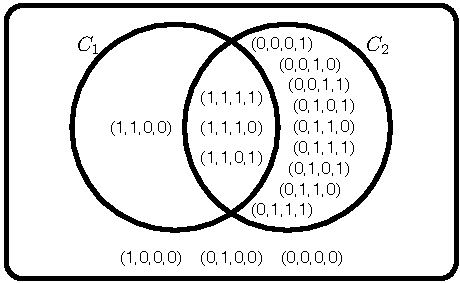
\includegraphics[scale=.7]{twoconcepts.pdf}&
	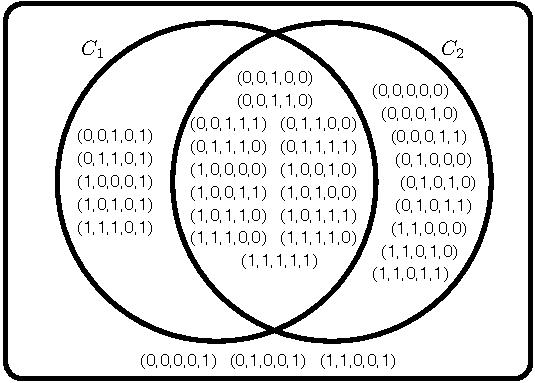
\includegraphics[scale=.7]{twoconcepts2.pdf}
	\\
	{\em a})&{\em b})
\end{tabular}
\end{center}\caption{\color{blue}Two toy examples of pair of concepts $C_1$ and $C_2$ with 4 and 5 features respectively. This is just a schematic illustration of where each element is placed with respect to concepts; note that 1) these concepts do not correspond to the ones used in the actual experiment (where 6 features are considered), and 2) elements in the actual experiment are not represented in this way (i.e.\ tuples of zeroes and ones). In {\em a}) concept $C_1$ can be described by $\varphi_1=p_1\land p_2$, and $C_2$ by $\varphi_2=p_3\lor p_4$. In {\em b}) concept $C_1$ can be described by $\varphi_1=(p_1 \land \lnot p_2) \lor p_3$, and $C_2$ by $\varphi_2=p_4\lor \lnot p_5$.
\color{black}}
\label{fig:twoconcepts}
\end{figure}
\sergio{Recalcar que en esta figura mostramos un ejemplo abstracto, y que en el experimento de verdad las cosas no se ven así.}

The actual experiment that we implemented consists of a sequence of 6 trials constructed in this manner. 
% During the experiment, we fix the semantics of all propositional features (i.e. their visual representation): a positive value of a $p_j$ is always represented by the same symbol, and its negative value is always represented by another symbol.
We now expand the 3 stages that compose the $i$-th trial of the experiment. \color{blue} For better understanding, see Figure~\ref{fig:trials}, with a schematic view of one trial. Notice that this figure is merely illustrative and does not aim to describe the details of a trial, but rather the sequence of phases and the logical flow within a trial. In particular, notice that the number of elements {\sf A}, {\sf B}, {\sf C} and {\sf D} are not meaningful, and they will vary in each trial of the actual experiment.\color{black} The actual concepts used in each trial is listed in Table \ref{trial_table}) and
more details of the actual implementation can be found in \S\ref{sub:experimentdetails} %\ref{Sec:AdditionalMethodology} 
 and \S\ref{FullExperimentDescription}.\santi{cambiar por nueva ubicacion}
 \color{black}
 
 \begin{figure}[t]
\begin{center}
	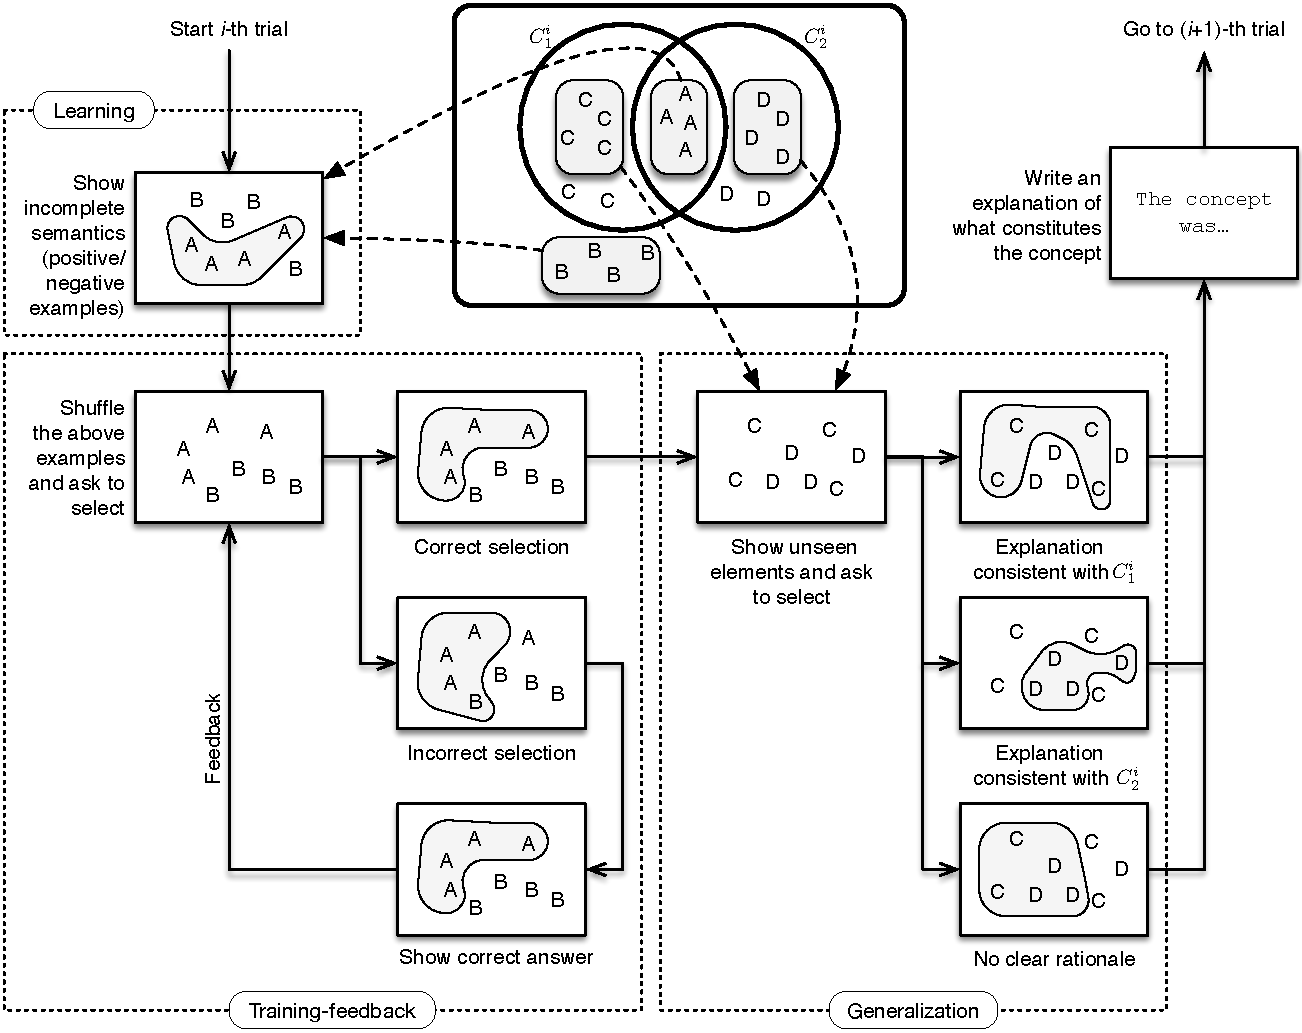
\includegraphics[scale=.7]{experimentscheme2.pdf}
\end{center}\caption{\color{blue}The scheme of our experimental framework for studying concept learning in the presence of multiple explanations. We illustrate the three phases that construct each trial: learning phase, training-feedback phase and generalization phase. Elements are represented with letters {\sf A}, {\sf B}, {\sf C} and {\sf D} (for example, the four letters {\sf A} in the intersection represent four different elements in the intersection). The depicted number of such letters {\sf A}, {\sf B}, {\sf C} or {\sf D} is irrelevant (for example, there would be 3 {\sf A}s for concepts of Fig.\  \ref{fig:twoconcepts}{\em a}), but 15 {\sf A}s for concepts of Fig.\ \ref{fig:twoconcepts} {\em b}).  \color{black}}
\label{fig:trials}
\end{figure}%\santi{corregi grafico - saque elementos B del complemento}
\sergio{Quizás recalcar en el caption que la cantidad de A,B,C,D mostradas es puramente ilustrativa. En realidad la cantidad de estas cosas depende de cada trial $i$. Quizás relacionar con la Figura 8, diciendo que las A son las cosas mostradas en verde, y las B las cosas que mostramos en rojo}

\begin{enumerate}
    \item \label{item:LearningStage}{\bf Learning stage.} The participant is exposed to a set of `in' elements corresponding to $C^i_1\cap C^i_2$ (marked as `{\sf A}' Figure~\ref{fig:trials}), and a set of `out' elements corresponding to the {\em complement} of $C^i_1\cup C^i_2$ (marked as `{\sf B}' Figure~\ref{fig:trials}). %Each valuation is tagged as `in' or `out'. Valuations tagged as `in' are in $C^i_1\cap C^i_2$, and valuations tagged as `out' are outside of $C^i_1\cup C^i_2$. Notice that this information is incomplete, in the sense that not all valuations are shown to the participant. In the illustrative example of Figure~\ref{fig:twoconcepts} only six valuations would be shown: the three `in' valuations in the intersection of $C_1$ and $C_2$, and the three `out' valuations outside of both $C_1$ and $C_2$.
    We call these shown elements `positive examples' and `negative examples', respectively. %\sergio{Cambié esto porque `in'/`out' puede confundir en que no queda claro si se refiere a algo visto por el participante o algo del diseño experimental. Igual dejé la mención de in/out para hacer referencia a este segundo sentido} 
    Notice that this information is incomplete, in the sense that not all possible examples are shown to the participant (as the only examples that are shown from $C^i_1\cup C^i_2$ are those in $C^i_1\cap C^i_2$). In the illustrative example of Figure~\ref{fig:twoconcepts}, only six elements would be shown: the three positive examples in the intersection of $C_1$ and $C_2$, and the three negative examples outside of both $C_1$ and $C_2$. The participant is asked to learn the concept represented by positive examples.

  As we prove formally in Appendix \ref{Sec:MainTheoremConcept}, the experimental design guarantees that there are only two %\footnote{Up to logical equivalence, since otherwise we would also consider things like $\tilde{\varphi}_1 = p_1\land p_2 \land p_2$.}
  propositional rules ($\varphi_1$ and $\varphi_2$ in Figure~\ref{fig:twoconcepts}), minimal over their respective sets of features, such that: \textit{(1)} they are \textit{consistent} explanations for shown examples (this is, they satisfy positive examples but do not satisfy negative examples), \textit{(2)} they use different features from each another (e.g.\ $(p_1, p_2)$ in $\varphi_1$ and $(p_3,p_4)$ in $\varphi_2$)  and, importantly, \textit{(3)} \textit{any} rule consistent with the examples must use a superset of the set of features of at least one of these minimal rules. For instance, in Figure~\ref{fig:twoconcepts} any rule that only uses $(p_2, p_3)$ cannot explain the examples, since $(1,\mathbf{1}, \mathbf{0},1)$ is a positive example but  $(0,\mathbf{1}, \mathbf{0},0)$ is a negative example. Any rule that can consistently explain the examples must mention a superset of $(p_1, p_2)$ (e.g.\  $(p_1, p_2, p_3)$) or a superset of $(p_3, p_4)$. The proof of this condition is shown in Theorem \ref{theorem:TeoremaPrincipal}, but we also illustrate here. In Figure~\ref{fig:twoconcepts}, observe that the negative example $(0,\mathbf{1}, \mathbf{0},0)$ was constructed from the positive example $(1,\mathbf{1}, \mathbf{0},1)$ by flipping the values of $p_1$ and $p_4$, and doing so results in an element that is inconsistent with both $\varphi_1$ and $\varphi_2$. When an alternative explanation leaves unused some features $p,q$ that appear in $\varphi_1$ and $\varphi_2$ respectively, there must be some element that satisfies both rules $\varphi_1,\varphi_2$, but none of them is satisfied when the value of $p$ and $q$ are flipped. Since the truth value of the alternative rule is maintained when features that do not appear in it change, and since we are showing as positive examples all elements that satisfy both rules $\varphi_1,\varphi_2$ and as negative examples all those that satisfy none of them, such alternative explanation must be inconsistent with the shown data.

  These three conditions guarantee that the experimental procedure illustrated in Figure \ref{fig:twoconcepts} is a logically sound method to present a concept consistent with two minimal rules chosen by the experimenter ($\varphi_1$ and $\varphi_2$), depending on which features the participant use to build the rule.
    

    \item {\bf Training-feedback stage.} The {\em same} examples of the learning stage are shown to the participant, but this time without indicating whether they are negative or positive and in a shuffled order. The participant is asked to tag each element as `in' or `out', in the same way they were tagged in the previous step. If all elements are classified correctly, the participant proceeds to the next stage. Otherwise, the participant is informed about the mistakes in their tagging, and after that the training-feedback stage starts again.
    
    \item {\bf Generalization stage.} {\em Previously unseen} elements are shown to the participant\footnote{With the exception of Trial 6, where one element is reshown in order to better test Hypothesis~\ref{Hip:FeatureBiasStickiness}. See \S\ref{sec:hypothesis}.}. These elements are taken from $C^i_1\setminus C^i_2$ and from $C^i_2\setminus C^i_1$ (here, `$\setminus$' denotes set difference). These elements are respectively marked as `{\sf C}' and `{\sf D}' in the scheme of Figure~\ref{fig:trials}. The participant is asked to identify those elements that correspond to the concept learnt in the learning stage. After they do so,  the next trial starts. If the participant selects those in $C^i_1\setminus C^i_2$, the concept learnt in the Learning stage was $C^i_1$, and if the participant selects those in $C^i_2\setminus C^i_1$, the concept they learned was $C^i_2$.
    Continuing with the example from Figure~\ref{fig:twoconcepts}, this process would allow us to determine if the participant was thinking in a rule with the features $(p_1, p_2)$ (namely, $\varphi_1$) or $(p_3, p_4)$ (namely, $\varphi_2$) to explain the concept. Of course, in practice the participant can select other elements, with no clear rationale.
    
    Once the participant chooses the elements, they are asked to write an explanation of what constitutes the concept; this answer is not part of the data analysis, except that it allows us to exclude participants that are using methods outside the scope of the experiment (such as taking pictures). Additionally, the written answers serve as an additional sanity check of whether the participants are actually thinking in a way consistent with the framework of propositional logic.
\end{enumerate}

More details of the experiment and its structure can be found in \S\ref{Sec:AdditionalMethodology} and \S\ref{FullExperimentDescription}.

\subsection{Experiment trials}\label{sec:hypothesis}
    The set of trials chosen in the experiment (Table~\ref{trial_table}) aims to reveal the biases that cause participants to choose one set of features over another in this framework where both sets of features have their own minimal rules consistent with the observed positive and negative examples. For instance, in Figure~\ref{fig:twoconcepts}, what causes participants to choose $(p_1, p_2)$ versus $(p_3, p_4)$ to explain the concept? Our hypothesis is that a key inductive bias is simply the frequency with which a subset of features was used previously to explain past concepts. We name this bias as \textit{feature stickiness}. %\sergio{``One of the authors' main findings regards "feature stickiness," the tendency to use features used to solve category learning problem N to also solve problem N + 1. Yet, this basic phenomenon was examined in work by John Kruschke testing the phenomenon of learned inattention (e.g., Kruschke \& Blair, 2000, PBR) in which features that are not useful for learning in phase N are then not used in phase N + 1 (i.e., subject "learned" that some features are not useful).''} % Kruschke, Kappenman, & Hetwick (2005, JEP:LMC) found that eye movements confirmed that attention was learned in the basic learned inhibition paradigm. Using somewhat more complex category structures, Hoffman & Rehder (2010, JEP:General) also found that eye movements revealed how an attention profile learned during a first phase of learning affected a second phase. Given that none of this previous work is discussed or cited it is unclear what the author's new contribution regarding feature stickiness is.


\renewcommand{\arraystretch}{1.4}
\newcommand{\marcaEnTabla}{{\bullet}}%\checkmark



\begin{table}[h]
\begin{center}
%   \begin{tabularx}{\linewidth}{|>{\centering\hsize=.5\hsize}X|>{\centering\hsize=.7\hsize}X| >{\centering\hsize=.70\hsize}X| >{\centering\hsize=.70\hsize}X| >{\centering\hsize=.9\hsize}X| >{\centering\hsize=.4\hsize}X| >{\centering\hsize=.4\hsize}X| >{\centering\arraybackslash\hsize=.4\hsize}X|}
%     \cline{1-8}
%     \multirow{2}*{\textbf{Trial}} &\multirow{2}*{\textbf{Groups}}& \multirow{2}*{$\mathbf{\varphi^1_i}$} & \multirow{2}*{$\mathbf{\varphi^2_i}$} & \multirow{2}{4\baselineskip}{\centering\textbf{Shown features}}  &\multicolumn{3}{c|}{\bf Tested hypotheses}\\\cline{6-8}
%     &&&&&\ref{Hip:AndOverOr}&\ref{Hip:FeatureBiasStickiness}&\ref{Hip:FeatureBiasTimeAdvantage}\\ 
%     \cline{1-8}
%     $i = 1$ &  A, B & $\varA \lor \varB$ 	& $\varC \land \varD $  & \multirow{5}*{$p_1$ to $p_6$} &$\marcaEnTabla$ & & \\ \cline{1-4} \cline{6-8}
%     $i = 2$&  A, B & $\lnot \varA \land \varB$ 					& $\varC \lor \lnot \varD$ 	 &   & & & \\    \cline{1-4} \cline{6-8}
%     \multirow{2}*{$i = 3$} & A & $\varA \land \varB$ 	& \mdl 15   &     \multirow{2}*{} & \multirow{2}*{} &&\multirow{2}*{$\marcaEnTabla$} \\\cline{2-4} 
%      & B & $\varE \land \varF$ 	& \mdl 15  &   &&&\\    \cline{1-4} \cline{6-8}
%     $i = 4$&  A, B & $ \lnot \varE \land \varF$ 					&  \mdl 15  &  &&&$\marcaEnTabla$\\    \cline{1-8}
%     $i = 5$&  A, B & $\varG \land \varH$					& \mdl 15  &  \multirow{2}*{$p_3$ to $p_8$}&&$\marcaEnTabla$&\\    \cline{1-4} \cline{6-8}
%     $i = 6$&  A, B & $\lnot \varG \land \lnot \varH$					& $\varC \land \varD$ &  &&$\marcaEnTabla$&\\    \cline{1-8}
%     \end{tabularx}

  \begin{tabularx}{\linewidth}{|>{\centering\hsize=.5\hsize}X|>{\centering\hsize=.7\hsize}X| >{\centering\hsize=.75\hsize}X| >{\centering\hsize=.75\hsize}X| >{\centering\hsize=.7\hsize}X| >{\centering\hsize=.3\hsize}X| >{\centering\hsize=.3\hsize}X | >{\centering\hsize=.3\hsize}X |>{\centering\arraybackslash\hsize=.3\hsize}X|}
    \cline{1-9}
    \multirow{2}*{\textbf{Trial}} &\multirow{2}*{\textbf{Groups}}& \multirow{2}*{$\mathbf{\varphi^i_1}$} & \multirow{2}*{$\mathbf{\varphi^i_2}$} & \multirow{2}{4\baselineskip}{\textbf{Shown \\ features}}  &\multicolumn{4}{c|}{\bf Tested hypotheses}\\\cline{6-9}
    &&&&&\ref{Hip:AndOverOr}&\ref{Hip:FeatureBiasStickiness}&\ref{Hip:FeatureBiasTimeAdvantage}&\ref{Hip:StickinessFeatureOperator}\\ 
    \cline{1-9}
    $i = 1$ &  X, Y & $\varA \lor \varB$ 	& $\varC \land \varD $  & \multirow{5}*{$p_1$ to $p_6$} &$\marcaEnTabla$ & && $\marcaEnTabla$\\ \cline{1-4} \cline{6-9}
    $i = 2$&  X, Y & $\lnot \varA \land \varB$ 					& $\varC \lor \lnot \varD$ 	 &   & & &&$\marcaEnTabla$\\    \cline{1-4} \cline{6-9}
    \multirow{2}*{$i = 3$} & X & $\varA \land \varB$ 	& \mdl 15   &     \multirow{2}*{} & \multirow{2}*{} &&\multirow{2}*{$\marcaEnTabla$} &\\\cline{2-4} 
     & Y & $\varE \land \varF$ 	& \mdl 15  &   &&&&\\    \cline{1-4} \cline{6-9}
    $i = 4$&  X, Y & $ \lnot \varE \land \varF$ 					&  \mdl 15  &  &&&$\marcaEnTabla$&\\    \cline{1-9}
    $i = 5$&  X, Y & $\varG \land \varH$					& \mdl 15  &  \multirow{2}*{$p_3$ to $p_8$}&&$\marcaEnTabla$&&\\    \cline{1-4} \cline{6-9}
    $i = 6$&  X, Y & $\lnot \varG \land \lnot \varH$					& $\varC \land \varD$ &  &&$\marcaEnTabla$&&\\    \cline{1-9}
    \end{tabularx}

\footnotetext{In the case of $i=3$ and group A, the MDL15 rule was $((\varC \lor (\varD \lor \varE))\land(\lnot\varC \lor((\varD \lor\lnot\varE)\land(\varE \lor \lnot\varD))))$} %Uso \footnotetext porque \footnote no funciona desde la tabla
\caption{The trials of the experiment. Here $\varphi^i_1$ and $\varphi^i_2$ represent the two competing concepts \color{blue} $C^i_1$ and $C^i_2$ \color{black} at the $i$-th trial (we denote each concept by the shortest propositional rule whose semantics describes the concept). By ``MDL15'' we denote a concept whose shortest rule is of length 15 (and made of three propositional symbols other than the competing rule in the corresponding trial, see Section \ref{Resultados:MDLbias} for details). In all trials the full universe size is $2
^6=64$, corresponding to all possible elements over 6 propositional features. We indicate how participants were divided into groups X and Y, which was used only for Hypothesis \ref{Hip:FeatureBiasTimeAdvantage}. We also indicate which features where shown in the examples, and which hypothesis where tested by the different trials.}
\label{trial_table}
\end{center}
\end{table}
\sergio{Hay que explicar un poco más en el texto por qué dividimos en 2 grupos ("The reader can be helped a bit here to explain this better the first time it is referred to (also pointing out why this important in the set-up")}
\sergio{Potencialmente se pueden poner 2 columnas más: ejemplos positivos mostrados, ejemplos negativos mostrados (en la learning phase)}

%\widesergio{Nota: es necesario que en los primeros dos aparezcan en el universo mostrado $\varE$ y $\varF$, para que no haya cuestiones de novedad para el groupo B en el i=3}

%\widesergio{Tratar de hacer más claras las explicaciones. ``This section needs a lot of work.''. Le dí una pasada}
%\widesergio{``The reader needs a complete description of what features were relevant in each phase in order to determine what confounds might have been introduced by this within subject design'' Este comentario es raro... la tabla es bastante clara. O ser\'a que quiere que se presente exactamente qu\'e valuaciones se pusieron? Traté de dejarlo más claro igual.}%; en el sentido que usar $p_j$ deja bien en claro las features de una manera que usar $C_j$, $D_j$ no. Por otro lado, quizás estaría bueno incorporar una notación general tipo: en este Trial, $C_1,C_2 = p_3, p_4$, y después referirse a esas features locales en vez de a las $p_j$? Igual es medio feo, porque en realidad serían $C^i_1$, $C^i_2$ }



\color{blue} We now present the main hypotheses of this work, and their relation with the various experimental trials. For the exact preregistered formulation of the hypotheses, see Section~\ref{Hypotheses}. \color{black}

\paragraph{Hypothesis \ref{Hip:AndOverOr}}
In Trial 1 we explored whether the same factors that determine rule learning difficulty when learned in isolation also determine participants which features participant use when explaining a set of examples consistent with two minimal rules. Particularly, it is well known %\sergio{ ``the authors find that learners prefer conjunctive versus disjunctive rules, a preference that the field has been aware of for decades.'... quizás hay que hacer más énfasis en que sabemos esto?}
that concepts involving logical conjunctions are learned faster than concepts involving logical disjunctions \cite{bourne1970knowing}. %\sergio{``However, Feldman (2000) has demonstrated that that learning difference can instead be explained by parity—the difference in the number of positive and negative examples of each rule. Indeed, there are fewer examples consistent with a conjunction as compared to a disjunction (4 vs. 12 during learning and 1 vs. 9 during generalization). Thus, it is unclear if the observed feature bias is due to a rule preference''. Leer Feldman 2000. Pero no entiendo. La cantidad de ejemplos positivos y negativos mostrados es igual para disyunción y conyunción }.
In Trial 1, the minimal consistent rule is a disjunction if the observed features are $(p_1, p_2)$, and a conjunction if the observed features are $(p_3, p_4)$. Importantly, unlike previously concept learning experiments, both the two-feature disjunction and conjunction are consistent with the observed set of examples. We hypothesize that the learning bias that causes the conjunction to be learnt more easily than the disjunction will also carry over to this framework were both explanations are possible (using different features). 
%determine which features the participant attends to when two explanations are possible (i.e. features $(p_1, p_2)$).
As explained before, we use the generalization stage of Trial 1 to determine if participants understood the concept using $(p_1, p_2)$ (corresponding to a disjunction) or using $(p_3, p_4)$ (corresponding to a conjunction).
%\sergio{``(Note: To test the conjunction-disjunction bias, the text and Figure 1 use p1 and p2 to refer to conjunction features and p3 and p4 to refer to disjunction features. However, those labels are reversed in Table 1. This is another example that makes the manuscript hard to follow)'' Es raro, porque el texto dentro del experimento usa la tabla... por las dudas aclar\'e que el ejemplo no corresponde a ningun Trial}



% \widesergio{Pensar cómo contar de esto. Más que nada es algo que analizamos sin mucha expectativa de que haya un efecto fuerte, pero que era interesante de todos modos interesante hacer el experimento para ver si lo había.}

\paragraph{Hypothesis \ref{Hip:FeatureBiasStickiness}.} 
    The \textit{feature stickiness} bias was tested in Trials 5 and 6 in the experiment. After participants have gained sufficient experience with the task, in Trial 5 participants encountered a set of examples consistent with two minimal explanations, a very simple one that uses features $(p_7, p_8)$ and a very complex one that uses $(p_4,p_5,p_6)$. This leads participants to explain the concept using $(p_7, p_8)$, or otherwise discover a very complex explanation. We hypothesized that most participants will select the features $(p_7, p_8)$.
    
        In the following concept (Trial 6), participants must choose between explanations that use the previously useful features $(p_7, p_8)$, or another fresh set of features $(p_3, p_4)$. We hypothesize that participants are more likely to explain the concept using $(p_7, p_8)$, only because these features were useful in the previous concept. Also, recall that explanations that use a set of features containing either $(p_7, p_8)$ or $(p_3, p_4)$ are also compatible. For example, in Trial 6 the explanation $p_3 \land p_4 \land \lnot p_7$ is compatible with the observed examples. We are also interested in these rules (e.g.\ we think it is more likely that participants will use $(p_7, p_8, p_3)$ than $(p_3, p_4, p_7)$). The seven elements chosen for the generalization stage of Trial 6 allows us to do precisely this: 7 elements appeared on the screen, with $p_3, p_4, p_7, p_8$ respectively equal to $(1, 1, 1, 1)$, $(1, 1, 0, 1)$, $(1, 1, 1, 0)$, $(1, 1, 0, 0)$, $(1, 0, 0, 0)$, $(0, 1, 0, 0)$, $(0, 0, 0, 0)$. These elements are respectively consistent with the minimal rules $p_3 \land p_4$, $p_3 \land p_4 \land \lnot p_7$, $p_3 \land p_4 \land \lnot p_7 \land \lnot p_8$, $p_3 \land \lnot p_7 \land \lnot p_8$, $p_4 \land \lnot p_7 \land \lnot p_8$ and  $\lnot p_7 \land \lnot p_8$. Importantly, none of the elements is consistent with more than one of the two minimal rules.
    
\paragraph{Hypothesis \ref{Hip:FeatureBiasTimeAdvantage}} 
We address the question of whether the feature stickiness bias represents a computational advantage in itself. More concretely, we ask if participants find a consistent rule {\it faster} when they are reusing the same features as in the previous trial.
We tested this question, independently of the effect of the feature stickiness bias, in Trials 3 and 4 of the experiment. In Trial 3, we separated participants into groups X and Y. In the same manner as in Trial 5, in Trial 3 group X was biased to learn the rule using $(p_1, p_2)$, and group Y using $(p_5, p_6)$. In the next trial (Trial 4), participants were biased to learn the rule using $(p_5, p_6)$. We hypothesized that participants from group Y will learn concept $C^4_1$ faster than participants from group X, given that they are reusing the same features they used in the previous trial.


 \paragraph{Hypothesis~\ref{Hip:StickinessFeatureOperator}} 
% \widesergio{Insertar imagen con la data de la transición Trial 1 a Trial 2}
 Another question, tested with Trials 1 and 2, examines the relative strength of feature bias versus operator bias. That is, we wanted to determine whether there is some strong effect that clearly biases attention towards features (or rather toward operators) that have previously been found useful for describing concepts. We tested this by switching the operator ($\lor$/$\land$) that each pair of features can use to form a useful rule in each trial, and by then comparing the number of participants that explained the shown examples of Trial 2 by reusing the same features from Trial 1 versus those that reused the operator but used different features.
 
% \bigsergio{ Pasado a Results
 %In this work, we did not find conclusive evidence regarding this hypothesis, so we decided to leave it out of the results report. %(but see Section~\ref{sec:Discussion} for discussion).  We believe that the cause was an experimental setup that underestimated the strength of the bias favoring the $\AND$ operator over the $\OR$ operator. A future experiment could probe the existence of operator stickiness by having longer consecutive periods where feature reutilization is not a useful bias and where only one logical operator remains useful for explaining a concept, before finally presenting a concept that can be explained via two different rules, each using different operators.
 % We leave for future work the task of studying the interaction between the feature stickiness bias and the precise structure of the logical rules being learnt. 
 %}
    
    
%%%%%%%%%%%%%%%%%%%%%%%% METHODOLOGY %%%%%%%%%%%%%%%%%%%%%%%%%%%%


\section{Methodology}\label{Sec:AdditionalMethodology}


\subsection{Preregistration and data}
This study's methodology, data collection procedures, sample size, exclusion criteria, and hypotheses were preregistered on the Open Science Framework (OSF) in advance of the data collection and analysis. The preregistration can be accessed at \url{https://osf.io/mgex3}, while the obtained data is available in \url{https://osf.io/gtuwp/}.

%\widesergio{Quiz\'as resaltar la importancia metodol\'ogica de hacer pre-registraci\'on}
%\widesergio{los p-values son con null hypothesis significance testing (NHST) de Fisher (¿cierto?), que solo tiene sentido usar si uno está testeando predicciones (y no hipótesis post hoc). Quizás recalcar que para esto es vital estar haciendo la pre-registración, como para remarcar su importancia.}

In this work we also make some exploratory (not preregistered) analyses: we corrected for verbal explanations that are not consistent with a positive interpretation of the concept for Hypothesis~\ref{Hip:AndOverOr}, we excluded outliers from the analysis in Hypothesis~\ref{Hip:FeatureBiasTimeAdvantage}, and we considered the effect of the participant's learning history  beyond the immediately previous trial in Hypothesis~\ref{Hip:FeatureBiasStickiness}. We also explicitly analysed, in this framework of multiple consistent explanations, the difference in revealed difficulty between rules of greatly differing minimal length.

%\subsection{Access to experiment data}
%\widesergio{Un link hacia los datos experimentales anonimizados? Notar que la info recopilada por el experimento ya es muy completa: menciona universo mostrado, elecciones hechas por participantes, tiempos, asignación de variables proposicionales a features, etc. Por ejemplo podemos hacer accesible el csv en -Categorization-data-FINAL, aunque notar que le puse muchos recordatorios y están en español.}


\subsection{Hypotheses} \label{Hypotheses}
%\pablo{Sacaria toda esta seccion. Mencionamos a las hipotesis mas adelante de una manera mas entendible.}
%\sergio{Me parece que deberían estar declaradas conjuntamente en algún lado, y no aparecer individualmente de formas poco referenciables. Tal vez se puede cambiar la presentación, o expandir el significado de cada una?}
The hypotheses were preregistered as follows: 

\begin{enumerate}[label=\Roman*]
    \item\label{Hip:AndOverOr} In a scenario of two possible explanations for a concept, one of which can be modeled by the logical \AND between two features and other which can be modeled by the \OR between two other features, most people will find the \AND explanation over the \OR explanation.% (Trial 1).     
    \item\label{Hip:FeatureBiasStickiness} If a person has used a set of features in the construction of an explanation for a concept, it is more likely that she will also find an explanation containing those features %(but they may also contain other features, as in this scenario there are multiple possible explanations) 
    in the following trial. % (Trials 5 to 6)
    \item \label{Hip:FeatureBiasTimeAdvantage} When a concept can only be reasonably described by a given set of features, a person will find this description faster if that same set of features was useful for her in the immediately previous trial.
    \item\label{Hip:StickinessFeatureOperator} In a scenario where both features and operators are repeated from a trial to the next, there will be a stickiness effect favoring one of them over the other.% (Trials 1 to 2).
\end{enumerate}


\subsection{Representational details}\label{sub:experimentdetails} 

%The experiment begins with the (hidden) assignment of the participant to one of two groups X or Y. Each participant will be exposed to 6 trials. The structure of each $i$-th trial is the same for each participant, except for $i=3$, where groups X and Y have different trials (see Table~\ref{trial_table}).
The underlying mathematical structure of the trials uses propositional variables, valuations, and sets of valuations. However, these are not shown abstractly, but rather are represented via correspondences to features (symbols), elements (boxes), and concepts (collections of elements). 
%Propositional features, valuations over them, and concepts are not represented in an abstract mathematical way, but via a correspondence between the propositional values and a set of visual symbols. 
We next describe details of the representations used for the experiment and its competing concepts.
%For a more detailed description of the experiment and its design, see the Appendices. %~\ref{FullExperimentDescription} and \ref{Experiment_design}.

\paragraph{Features\textemdash propositional variables}
The experiment encompasses eight propositional variables: $p_1,\dots,p_8$. Each variable can take one of two possible values, and these values are graphically represented by icons. \color{blue} For instance, $p_1$ can be assigned icon `A' or icon `B', representing the values 1 (positive) and 0 (negative) respectively, $p_3$ can be assigned a `$+$' icon or `$\times$' icon  representing 1 and 0 respectively, and so on. \color{black}
%For instance, $p_1$ can be assigned icon `$+$' or icon `$\times$', representing 1 and 0 respectively, $p_2$ can be assigned a `sun' icon or `moon' icon  representing 1 and 0 respectively, and so on.
Figure~\ref{Figure:references} shows the pairs of values for each of the eight propositional variables. The assignment of pairs of icons to propositional variables is randomized at the start of the experiment, and does not vary within the experiment. 
The reason to choose icons instead of (colored) values 0,1 is to avoid the possibility of mentally learning a concept using `counting' or other operators not present in propositional logic. For example, using $\{0,1\}$ values, a possible explanation for a concept could be {\em more than 3 ones}, but such a description would be impossible in the icon-based representation, since different propositional variables have no values in common. See \S\ref{Experiment_design} for more details on these design considerations.

\begin{figure}[h!]
\begin{center}
    	\includegraphics[scale=2]{Features8.png}
	\caption{Pictured above are the features, the visual representation of the positive and negative values of the propositional variables. The upper row represents positive values of the propositional variables, while the lower row represents their negation.}
	 \label{Figure:references}
\end{center}
\end{figure}


\paragraph{Elements(boxes)\textemdash valuations} A valuation over the propositional variables is visually represented as a square/box with the values (icons) of all propositional variables set at random positions inside the square. See Figure~\ref{Figure:element} for an example of such an element. The reason for choosing this representation is to avoid directional biases that could influence learning, and to exclude ordering and other operators from the language of thought (see \S\ref{Experiment_design} for more details on these considerations). % from the natural order of $p_1,\dots,p_8$ in the language of thought. %, and perhaps using it for memorizing. %For example, using tuples for representing valuations, a concept could be explained as {\em sun, then `A'}. Such explanation is impossible in the actual icon-based random-position setting.
Each time an element is shown (in particular, within the loop in the training-feedback) a new random position is chosen for the propositional features inside it.
%

\begin{figure}[h!] 
\begin{center}
    	\includegraphics[scale=0.6]{BordeNeutro.PNG}
	%\caption{An example of a valuation, in pictographic language.}
	\caption{An element. This box containing features is the visual representation of a valuation over six propositional variables. Here the box appears with a neutral border, but boxes in the experiment always appear with a border that denotes whether they are positive or negative examples. The position of the symbols is irrelevant for the concepts, and is randomly assigned.}
	\label{Figure:element} 
\end{center}
\end{figure}


\paragraph{Undetermined concepts\textemdash sets of positive/negative valuations}\label{IncompleteConcepts} The concept shown in the learning stage of a trial corresponds to two non-overlapping sets of valuations, and these two sets do not cover all possible valuations. This is represented as a sequence of `in' and `out' elements, with no information given on elements that are not shown. % (that does not show all possibilities). 
At the learning stage, shown `in' elements (positive examples) are represented as a green box and shown `out' elements (negative examples) as a red box. See Figure~\ref{Figure:training} for an example of a tagged sequence of elements used in the learning stage. Each time the concept is presented, we shuffle the order in which their positive and negative examples are shown, but always presenting all positive examples first (also, each valuation is assigned new random positions for the features inside the corresponding box). 

%The purpose of placing the positive examples first is to bias the participant into thinking of the concept by its positive formulation, instead of possibly thinking of a rule that would describe the negative examples, and then negating that rule to obtain the positive one. This is important when we want to reason about the ease of learning different operators: by default we assume %\footnote{This assumption has been verified by checking the verbal explanations of the participants in the generalization phase} that participants that correctly select positive examples of the concept are thinking the positive rule, which differs in its operator from the negative rule (by the De Morgan laws). 
%

\begin{figure}[h!] 
\begin{center}
    	\includegraphics[scale=0.4]{Learning.PNG}
	%\caption{An `in' (green) and `out' (red) tagging example in a learning stage.}
	\caption{A sequence of positive and negative examples in a learning stage, corresponding to Trial 1.  A green border informs the participant that the element belongs to the concept, while a red-bordered one informs that it does not belong to the concept. In this case, the examples could be explained as either `boxes containing both an upwards pointing arrow and a question mark' or as `boxes that contain a circle or a plus sign', but note that these two rules determine different concepts over the complete set of possible elements.}
	\label{Figure:training} %Corresponde al Trial 1
\end{center}
\end{figure}

\paragraph{Hidden concepts/rules\textemdash formulas}
Over the full set of valuations, a concept is simply the set of valuations that positively describe it. The two hidden concepts for each trial correspond to the valid and minimal generalizations that can be made from the incomplete concepts. They can be described as the semantics of the two propositional formulas (rules) that can be used to explain the incomplete concept (see Table~\ref{trial_table}); while these rules coincide over the incomplete universe shown in the learning stage, they differ over the set of all valuations. For more details, recall the beginning of Section~\ref{Subsec:ExperimentFlow} and its Item~\ref{item:LearningStage}. 

%\widesergio{En general, tuve más cuidado con hablar de "concept". Se usaba ambiguamente para referir al universo mostrado y a generalizaciones. En general aclaré con "incomplete" o undetermined a lo que corresponde con lo que se ve en la learning fase. Está bien? Acá uso el término de Hidden concepts para recalcar que el participante nunca está seguro si su teoría está bien o no, y porque es en realidad en base a estos conceptos que creamos el universo a mostrar}


%%%%%%%%%%%%%%%%%%%%%%% DETAILS EXPERIMENT %%%%%%%%%%%%%%%%%%%%%%
\subsection{Details of the experiment's structure} \label{FullExperimentDescription} 
As we explain in Section~\ref{Section:Experiment}, each instance of the experiment consists of 6 trials where the participants must learn a concept from an incomplete universe. The presented positive and negative examples are such that there are exactly two minimal rules (up to logical equivalence) in propositional logic that 1) are consistent explanations for the shown examples 2) use disjoint sets of variables from each another 3) any rule consistent with the examples must use a superset of the set of features of at least one of these minimal rules. 
This experimental setup will allow us to distinguish which of these rules best represents the way that the participant learned the concept. See \S\ref{Sec:MainTheoremConcept} for technical details.

%\textit{(1)} they are \textit{consistent} explanations for shown examples (this is, they satisfy positive examples but do not satisfy negative examples), \textit{(2)} they use different features from each another (e.g. $(p_1, p_2)$ in $\varphi_1$ and $(p_3,p_4)$ in $\varphi_2$)  and, importantly, \textit{(3)} \textit{any} rule consistent with the examples must use a superset of the set of features of at least one of these minimal rules.



Observe that merely asking the participant to select already seen elements does not give us any obvious insight into the internal process that derived into the learning of the concept; even if they internalized the concept using one of the two rules, it would remain uncertain which one they used, as both rules have the same semantics over the shown universe. %at the very least, they could have internalized the concept using a representation akin to either of the two rules. 
In order to distinguish between these two cases, we use a generalization stage where previously unseen elements of the universe are shown, and the participant must select those that they believe belong to the concept. Of these new elements, some are consistent with only one of the rules, and other are consistent only with the other rule\footnote{The Trial 6 is an exception, and has an element that is consistent with both rules.}. Furthermore, immediately afterwards we ask for a written explanation of what characteristics the participant thinks describe the  concept.

Structurally, the experiment begins with the (hidden) assignment of the participant to one of two groups X or Y (see Table~\ref{trial_table}) and the exposition to a page with instructions. 
Afterwards, there are 6 trials with the following structure: they begin with a learning stage; they continue to a training stage where they get feedback if they fail to correctly select the elements that belong to the concept; a generalization stage where they must choose between elements of the universe that were not shown previously; and, in all but the last trial, a stage where the participants can rest between trials.

%For notes on the experiment design, see Section~\ref{Experiment_design}.

We are now going to describe each of these stages plus the introductory page, with a greater detail than that of Section~\ref{Subsec:ExperimentFlow}.

\subsubsection{Introduction and explanation}
This is the page that subjects are shown at the beginning of the experiment. It describes the main task they will be asked to perform: that of learning from examples to distinguish what kind of `boxes' belong to a certain concept. These elements are represented as a collection of 6 symbols, no more than one from a same pair. It is also informed that the position of the symbols does not matter. See Figure~\ref{Figure:element} for an example element.

%\begin{figure}[h!] 
%\begin{center}
 %   	\includegraphics[scale=0.6]{Images/BordeNeutro.PNG}
%	\caption{(A closer look to Figure~\ref{Figure:valuation}) An example box with a neutral border (in the experiment, boxes always appear with a border that denotes whether they belong to the current concept or not). The position of the symbols is irrelevant for the concepts, and is randomly assigned.}
%	\label{Figure:Element} 
%\end{center}
%\end{figure}

When the subject indicates they have finished reading the instructions, they are sent to a fullscreen page with three multiple-choice questions whose purpose is to verify that the participant has understood the instructions; if they miss some answer, they are returned to the previous page and the cycle is repeated until they succeed.

If the participant answers correctly, they are now ready to begin, and the phases~\S\ref{Subsection:learning}, \S\ref{Subsection:training}, and \S\ref{Subsection:generalization} are then entered sequentially for each of the 6 trials.

\subsubsection{The learning phase}\label{Subsection:learning}
In this phase of a Trial $i$, the participant is shown a set $S^i \subsetneq U^i$, a proper subset of elements from the current universe. Each universe syntactically corresponds to all the combinations of truth values for 6 propositional variables taken from the set $\{\varA, \varB, \varC, \varD, \varE, \varF, \varG, \varH\}$, thus spawning a set $U^i$ of 64 elements. On the semantic side we call `features' the visual representations of the propositional variables, and these representations remain fixed through the experiment (recall Figure~\ref{Figure:references}).
%\begin{figure}[h!]
%\begin{center}
    %	\includegraphics[scale=2]{Images/Features8.png}
	%\caption{Pictured above are the features, the visual representation of the positive and negative values of propositional variables. The upper row represents positive values of the propositional variables, while the lower row represents their negation.}
	 %\label{Figure:Features}
%\end{center}
%\end{figure}
The elements of $S^i$ are shown as boxes, some of which have green border (denoting a positive example, that the element belongs to the concept), while the rest have red borders (denoting a negative example, that they do not belong).
The green-bordered boxes are shown first, with the red-bordered ones appearing after the last box with green border. 
%\sergio{ Podríamos recalcar que primero se muestran las verdes (los ejemplos positivos) y se seleccionan los positivos. Esto es importante porque la categoría puede también aprenderse viendo su negación, donde el $\lor$ pasa a ser un $\land$ y viceversa... también podemos aclarar que todos contestan con la formulación "positiva", de acuerdo a las explicaciones verbales} 
See Figure~\ref{Figure:training} for an example learning set. 
%\begin{figure}[h!] 
%\begin{center}
 %   	\includegraphics[scale=0.4]{Images/Learning.PNG}
%	\caption{(A closer look to Figure~\ref{Figure:concept}) A complete learning set, corresponding to Trial 1. A green border informs the participant that the element belongs to the concept, while a red-bordered one informs that it does not belong to the concept. In this case, the examples could be explained as either `boxes containing both an upwards pointing arrow and a question mark' or as `boxes that contain a circle or a plus sign'.}
%	\label{Figure:Training} %Corresponde al Trial 1, pero podria ser del 2 si uno no se fija que las asignaciones de positivo y negativo estan fijas.
%\end{center}
%\end{figure}

If the graphical representations are abstracted away to the underlying basic structure, there are two propositional rules $\varphi^i_1$ and $\varphi^i_2$ (of minimum length in their class of logically equivalent rules, see Table~\ref{trial_table}) whose semantics correctly classify the positive and negative examples shown. If we call $C^i_1, C^i_2$ the sets of valuations that satisfy $\varphi^i_1, \varphi^i_2$, respectively, we have that $S^i = (C^i_1 \cap C^i_2) \cup \overline{(C^i_1 \cup C^i_2)}$. The rules $\varphi^i_1, \varphi^i_2$ use at most\footnote{The rules that are actually `learnable' use exactly 2 propositional variables.} 3 of the 6 propositional variables available in $U^i$, and the two rules do not have propositional variables in common. 

When the participant believes they have learned which elements belong to the concept, they can click a button to proceed to the next stage.

\subsubsection{The training\textendash feedback phase}\label{Subsection:training}

In this phase, the participant is shown a random rearrangement of $S^i$, with all the elements now surrounded by a red-bordered square. % (which signifies that the element does not belong to the concept).
The subject must click exactly those elements (if any) they believe belong to the concept \textemdash changing them to a dotted green border (see Figure~\ref{Figure:ElementSquares})\textemdash and then has to click a button to submit their choice.

\begin{figure}[h!] 
\begin{center}
    	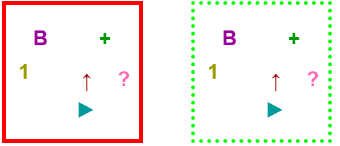
\includegraphics[scale=0.6]{SelectionSeparadosIguales.png}
	\caption{An unselected element, to the left, is represented by solid red borders. The same element in a selected state, to the right, is indicated by dotted green borders.}
	\label{Figure:ElementSquares}
\end{center}
\end{figure}

If their selection was incorrect, the participant is shown which elements they misclassified (either by clicking them incorrectly or by failing to click them, see Figure~\ref{Figure:Misclassifications}). When they click a button to continue, they restart this stage (with a fresh randomization).

\begin{figure}[h!] 
\begin{center}
    	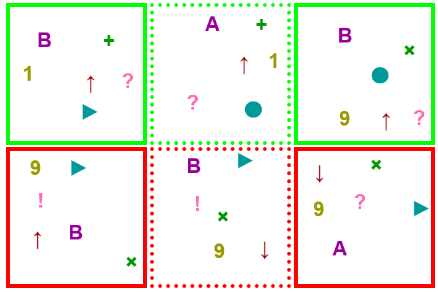
\includegraphics[scale=0.5]{FeedBack2SeleccionParcial.PNG}
	\caption{A partial section of the feedback resulting from a wrong selection. A solid green border means that the box was correctly selected as belonging to the concept. A solid red border means that it was correctly left unselected, meaning that it did not belong to the concept. A dotted green border means the box belongs to the concept but was not selected, and a dotted red border means that the box does not belong to the concept but was selected.}
	\label{Figure:Misclassifications}
\end{center}
\end{figure}

When the participant finally makes the correct selection, they continue to the next phase. 

\subsubsection{The generalization phase}\label{Subsection:generalization}

In this phase, the participant is shown a subset of $U^i \backslash S^i$ (namely, in $(C^i_1 \cup C^i_2) \backslash (C^i_1 \cap C^i_2)$), that is, a selection of elements that were \emph{not} present in the learning phase (hence nor in the training phase). The participant must classify which of these elements they think belong to the concept. The participant does not receive feedback on the choices they make here. Except for the sixth trial, part of these elements satisfy the rule $\varphi^i_1 \land \lnot \varphi^i_2$, while the rest satisfy $\varphi^i_2 \land \lnot \varphi^i_1$. %\sergio{Excepto en el \'ultimo trial, donde permitimos cualquier combinación válida de los 4 conyuntos (lo que nos da 7 posibilidades)}.
Thus \textemdash assuming the participant learned the concept via a process akin to a representation of one of the two rules\textemdash\, this phase crucially serves to distinguish which rule they have learned, if any.

After this selection, the participant is asked to submit a written explanation of what characteristics they think constitute the concept. This written explanation serves as an additional validation of whether they are thinking in a way describable by propositional logic according to our assumptions, or if rather they are using other methods (memorization, pen and paper, screenshots, other logics or formalisms, etc.). 

%%%%%%%%%%%%%%%%%%%%%%%% NoTES EXPERIMENT DESIGN %%%%%%%%%%%%%%%%%%%%%%%%%%%%


\subsection{Notes on the experiment design}\label{Experiment_design}
\widesergio{Quizás mejor dejarla en Apéndice esta subsection}

The elements, universes, and rules that constitute our experiment were devised in terms of propositional logic. However, it is important to be careful with the semantics, i.e.\ the way elements are actually shown to the participants. We have to avoid giving more salience to the semantics of a propositional variable over the others, and it is imperative to select the semantics of variables in a way such that they do not share characteristics that might escape our propositional grammar: for example, if the propositional variables were represented as circles that can be distinctly colored or not, it would be quite natural to assume that counting colored or uncolored circles could provide information, but this option is not considered in a theoretical design that assumes only propositional operators to describe rules. A related consideration is that we must also avoid introducing other regularities extraneous to the propositional formulation: if the images corresponding to all propositional variables are always shown in a straight line in the same order, salience effects might appear \emphstyle{even if} we avoid semantics that become more expressive thanks to the ordered nature of the represented variables (such as with descriptions of the form {\em the first and last elements are of the same size}).%that permit unwanted descriptions such as `the first and last elements are off'.

\paragraph{Building adequate semantic representations for our logic.}
Taking these precautions into account, we chose to match each propositional variable with a particular image or figure, whose position in a square would be randomized (but avoiding superpositions). It was harder to decide exactly what would be the matching, but we finally decided to match each propositional variable with a set of two related Unicode characters (such as a triangle when the variable is $0$, and a circle otherwise). See Figure~\ref{Figure:references} for the exact representations. We took care to choose different types of characters for different variables: having $A,B$ for $\varA$ and $Y,Z$ for $\varE$ was out, since it naturally introduced counting of the type `there is no more than 1 letter' and the like.
Of course, this process is not fail-safe, as there are countless possible semantics associations that could introduce extra-propositional grammar into the experiment. But we tried to minimize the chance that this would happen easily or naturally, and assumed\sergio{Correctly? O sea, comentar algo?} that the written explanation stage would serve to catch these exceptions if they occurred.

Finally, to minimize possible salience effects from showing symbols that could have (despite our intentions to the contrary) different levels of conspicuousness, we randomized on a per-participant basis the assignment between pairs of symbols and propositional variables (but we didn't randomize the assignment to the positive or negative value of a variable; the same Unicode characters were always positive in all randomizations, or always negative).

\paragraph{Ordering of positive and negative examples.}
As mentioned before, in the learning stage we shuffle the order in which their positive and negative examples are shown, but always presenting all positive examples first.

The purpose of placing the positive examples first is to bias the participant into thinking of the concept by its positive formulation, instead of possibly thinking of a rule that would describe the negative examples, and then negating that rule to obtain the positive one. This is important when we want to reason about the ease of learning of different operators: the default assumption is %\footnote{This assumption has been verified by checking the verbal explanations of the participants in the generalization phase}
 that participants that correctly select positive examples of the concept are thinking the positive rule, which differs in its operator from the negative rule (by the De Morgan laws). 
%



%\subsubsection{The construction of trials}
%\widesergio{Completar con los propósitos que tiene cada trial? O queda esto ya dicho en otras secciones?}

%\subsection{Discussion of the main results (pasar a la otra secci\'on lo necesario y comentar esto)}\label{subsection:mainResults}

%\widesergio{Poner posibles interpretaciones de resultados. Sobre posibles problemas metodol\'ogicos, uno puede hablar de qu\'e tan adecuado fue nuestro lenguaje utilizado en base a respuestas escritas de participantes.
%Mencionar participation bias?
%Recordar \cite{crump2013evaluating}, que al menos muestra un contexto en el cual ser an\'onimo no parece reducir de forma agregada la confiabilidad en los datos obtenidos; y tener en cuenta que parecer\'ia que muchos abandonan estos problemas de categorizaci\'on, y de los que no lo hacen un porcentaje importante (20\%?) admite haber usado l\'apiz y papel}

%We think that our experimental setup for testing Hypothesis~\ref{Hip:StickinessFeatureOperator} was too weak. We believe that the prior favoring the AND operator over the OR operator is too strong, and overshadows possible effects of operator/feature stickiness in our two-trial test. A more robust experimental setup should be devised in order to deal with the issues of prior biases favoring different operators. 
%A more robust experiment design to test feature versus operator stickiness could consist of a sufficient number of trials in which the same combination of 

%\widesergio{También hablar de los resultados respecto a Hypothesis~\ref{Hip:AndOverOr} \ref{Hip:FeatureBiasTimeAdvantage} \ref{Hip:FeatureBiasStickiness}}


%\widesergio{ Only participants that successfully completed all trials had their data considered for this experiment. This could have potentially introduced some survivorship bias, but this problem would be more troublesome for other kind of experiment with more complex formulas (which would require more heavily that participants have the inclination to think in classical logic).}
% \widesergio{Volver a mencionar papers sobre qu\'e tan buena es la población de MTurk? Puesto en footnotes antes}



%%%%%%%%%%%%%%%%%%%%%%%% RESULTS %%%%%%%%%%%%%%%%%%%%%%%%%%%%

%!TEX root = main.tex

\section{Results}\label{Results}


\subsection{Hypothesis~\ref{Hip:AndOverOr}}\label{Results:AndOverOr}
We asked whether the conjunction-disjunction bias (which is known to affect learning times in the case of a single explanation \cite{bourne1970knowing}) also determines which features are used to describe a concept when two alternative explanations are consistent with the observed universe. In the first trial, the observed examples were consistent with $p_1 \vee p_2$ and with $p_3 \wedge p_4$. As explained in Section~\ref{Subsec:ExperimentFlow}, in the generalization stage we can determine if participants explained the concept using $(p_1,p_2)$ or $(p_3,p_4)$. We found that 77 of the 100 participants attended to $(p_3,p_4)$, which corresponds to an explanation that uses a conjunction. 11 participants attended to $(p_1,p_2)$ (corresponding to the use of a disjunction for the explanation), and 12 participants selected examples in the generalization stage inconsistent with both $p_3 \wedge p_4$ and $p_1 \vee p_2$. The probability of obtaining the difference between the number of participants that used $(p_3,p_4)$ and $(p_1,p_2)$ under the null hypothesis of randomly choosing between them is $P<10^{-12}$. 

Note that it is in principle possible that the participant learns the concept with a reverse interpretation of positive examples (A's in Fig. \ref{fig:trials}) and negative examples (B's in Fig. \ref{fig:trials}) (i.e. interpreting positive examples as negative and vice versa). As we mention in \S\ref{Experiment_design}, we induced a bias to understand the concept in the appropriate way by first presenting the positive examples in the learning phase and by asking them to click on the positive ones in the training phase. We note, however, that 9 participants gave verbal explanations consistent with focusing on the negative examples. For this trial, a reverse interpretation is problematic since the negation of a conjunction corresponds to a disjunction, and the negation of the disjunction to a conjunction (i.e. `$p\land q$' is logically equivalent to `$\lnot(\lnot p\lor \lnot q)$'). Thus, a more comprehensive analysis should take into account participants' verbal explanations in this trial. However, even considering the worst-case scenario in which these 9 participants were originally regarded as part of the `conjunction' group and they are now considered part of the `disjunction' group, the conjunction-disjunction bias is still significant ($P<10^{-7}$). We therefore conclude that, in this framework where multiple explanations are possible depending on the attended features, there is a bias favoring conjunctive explanations over disjunctive explanations. %\sergio{Acá o antes hay que discutir sobre la explicación alternativa de Feldman 200 que nos dijo un reviewer?}
%conjunction-disjunction bias determines which features of the objects participants attend to in this framework where multiple explanations are possible depending on the observed features.


\subsection{Hypothesis \ref{Hip:FeatureBiasStickiness}}\label{Results:FeatureBiasStickiness}   
Most participants understood the concept in Trial 6 using the same features $(p_7,p_8)$ used to describe the concept in Trial~5, even when the logical structure of the rule was exactly the same independently of attending to $(p_7,p_8)$ or to $(p_3,p_4)$. To show this, we study participants' choices in the generalization stage of Trial 6 (see Figure~\ref{fig:results1}). 

Suppose that a participant is thinking of %a rule logically consistent with
the rule 
$\lnot p_7 \land \lnot p_8$, thus they are only attending to features $(p_7,p_8)$ while ignoring the features $(p_3,p_4)$. Since $(p_3,p_4)$ are being ignored, the participant should mark those elements in which $(p_7,p_8)$ agrees with the rule $\lnot p_7 \land \lnot p_8$, irrespective of the values of $(p_3,p_4)$. That is, the participant should mark the elements with $(p_3,p_4,p_7,p_8)$ equal to $(0,0,\textbf{0,0})$, $(1,0,\textbf{0},\textbf{0})$, $(0,1,\textbf{0},\textbf{0})$ and $(1,1,\textbf{0},\textbf{0})$. These elements have $(p_7,p_8)$ equal to $(0,0)$ and `anything' for $(p_3,p_4)$. On the other hand, if the participant is thinking of the rule $p_3 \land \lnot p_7 \land \lnot p_8$, then she is attending to $(p_3,p_7,p_8)$, and she should mark $(\textbf{1},0,\textbf{0},\textbf{0})$ and $(\textbf{1},1,\textbf{0},\textbf{0})$. 

In general, by studying which of the 7 examples shown in Figure~\ref{fig:results1} (left) the participant selects in the generalization phase, we can deduce which features they were attending to (Figure~\ref{fig:results1}, right). For example, all participants should mark the example with $(p_3,p_4,p_7,p_8)$ equal to $(1,1,0,0)$, since it is consistent with all the logical rules irrespective of which features are used. %\sergio{y todavía más concretamente, vieron a ese ejemplo exacto en la learning stage}.
Indeed, as shown in Figure~\ref{fig:results1} (left), all participants selected this example. Although in practice the participant can select any of the 7 examples in the generalization stage, we found that all but five participants respected the rules of coherence illustrated in the previous paragraph. These 5 participants were `one example away' of respecting the rule, however, we leave them out of the feature stickiness analysis, but including them does not change our conclusions. The grey lines in Figure~\ref{fig:results1} (left) show simulations of agents that randomly select one of the seven possible subsets of features, and then proceed to select the examples consistent with the logical rule using that features. Participants responses (black line) are biased towards explanations using $(p_7,p_8)$, as predicted by the feature-stickiness bias. This can also be seen in  Figure~\ref{fig:results1} (right), after inferring which features participants used to build the rule for the concept. In addition to being biased towards $(p_7,p_8)$, several participants explained the concept using all available features $(p_3,p_4,p_7,p_8)$. This shows that, in addition to the feature stickiness bias, when the number of features is relatively small participants are also biased to describe the concept using all available features.

To quantify the feature stickiness bias, we assign a score to each participant according to the attended features in Trial 6 (deduced from the marked examples). The scores for the subsets $(p_7,p_8)$, $(p_3,p_7,p_8)$, $(p_4,p_7,p_8)$, $(p_3,p_4,p_7,p_8)$, $(p_3,p_4,p_7)$, $(p_3,p_4,p_8)$ and $(p_3,p_4)$ are 1, 2/3, 2/3, 1/2, 1/3, 1/3 and 0 respectively\footnote{Part (d) of the Analysis Plan section in our preregistration had a mistake in the use of features names: the learnable concept corresponding to the fifth trial uses $p_7$ and $p_8$, not $p_3$ and $p_4$ as erroneously written in that part; compare with the section on Study design, which matches Table~\ref{trial_table}.}. The average score for the 95 participants was 0.68 ($P<10^{-6}$ in a permutation test with the null hypothesis of randomly attending to one of the seven subsets of features, which correspond to the grey lines in Figure~\ref{fig:results1}), indicating a significant effect of the feature stickness bias. Although the feature stickiness bias was significant for both groups independently (Group X: average score 0.62, $P<10^{-5}$;  Group Y: average score 0.74, $P<10^{-6}$), we found that feature stickiness was higher in Group Y (two-sample t-test comparing the scores of the two groups shows $t=2.35$,  $P<0.05$). The only difference between the groups is that Group Y had already (artificially) experienced feature stickiness between the previous Trials 3 and 4, so they have already identified it as an useful bias for the task. This suggests that the entire concept-learning sequence can be important when studying learning biases. %even concepts learnt several trials in the past.

\begin{figure}
\begin{center}
	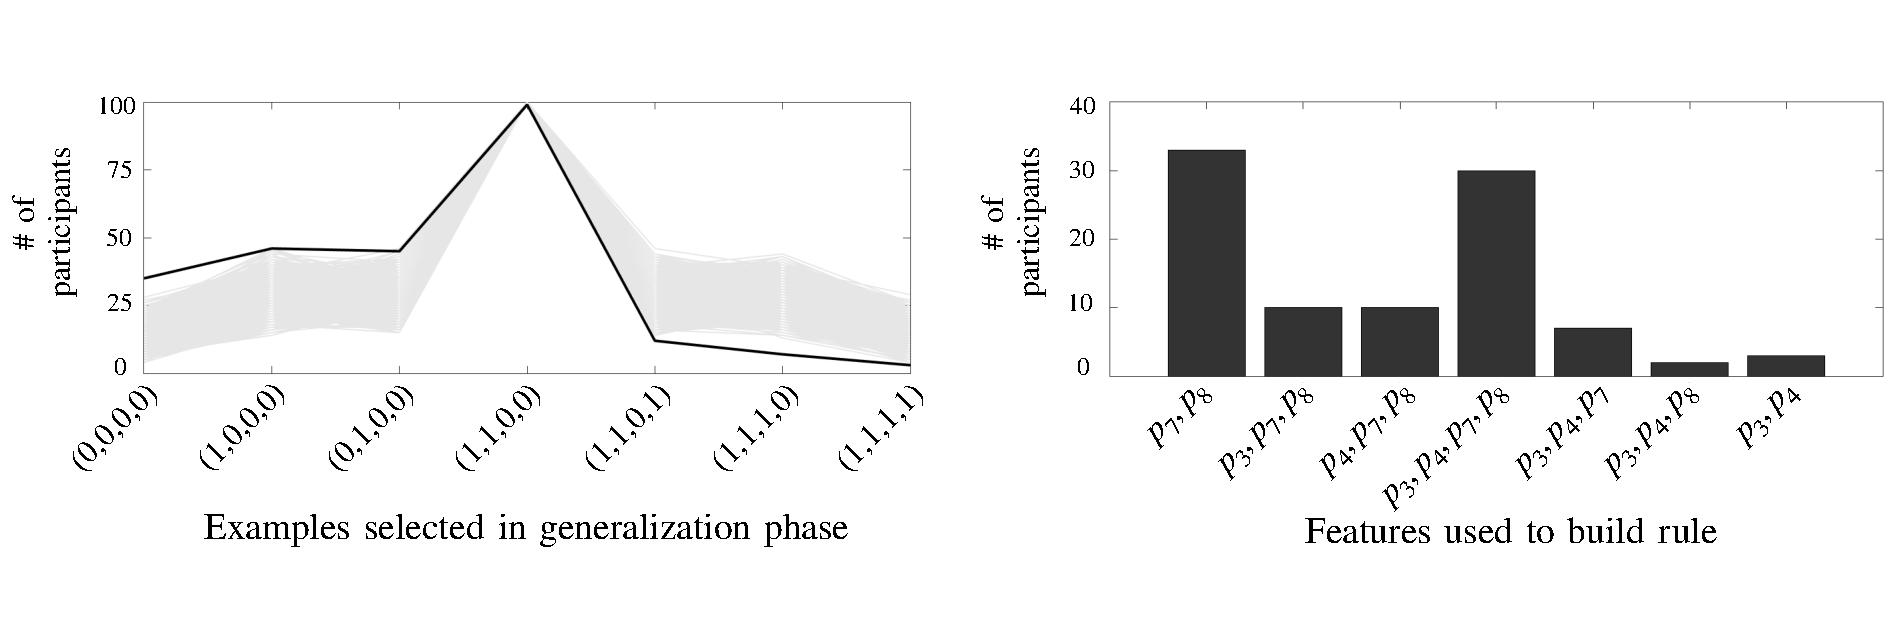
\includegraphics[scale=.47]{results_1.pdf}
\end{center}\caption{\textbf{(Left)} Number of participants (100 participants total) that, in the generalization stage of Trial 6, selected an element (possibly among others; the numbers add up to more than 100) with the elements written on the x-axis, indicating the values of the features $(p_3,p_4,p_7,p_8)$ respectively. As multiple choices were possible, the sum for all choices adds up to a value greater than 100. In grey we show 100,000 simulations in which 100 agents randomly attend to one of the seven subset of features (see text). \textbf{(Right)} From the selected objects in the generalization phase we can infer which features participants used to build the rule for the concept (95 valid participants, see main text).}
\label{fig:results1}
\end{figure}
%\sergio{Quiz\'as separar el gr\'afico de barras los 2/3 y 1/3 en sus dos valuaciones constituyentes, de modo que sea un histograma de la frecuencia de cada una de las 7 explicaciones}
 %\widesanti{caption de Figure estamos llamando example a algo que es un concepto o rule. Ademas, no se entiende por que 100. Lo hablamos, pero habria que aclarar. se trata de elecciones compatibles con la explicacion}
% \widesergio{``One comment about Figure 3: The authors assigned each participant a score indicating the proportion of old features that participants used during the generalization phase, with a higher score associated with higher bias in feature stickiness. Ideally, higher scores would be monotonically associated with more participants. But although the mode of the distribution was centered at the highest score, the relationship is not monotonic. This discrepancy is not discussed.'' Clarificar/explicar.}
 


%\sergio{Quiz\'as ac\'a se puede hacer referencia al \'unico analisis exploratorio que mencionamos a priori en la preregistracion: We also want to analyse stickiness using all the previous history of the subject instead of only the previous trial, although we may lack the power to find effects.}
 
 \begin{figure}
\begin{center}
	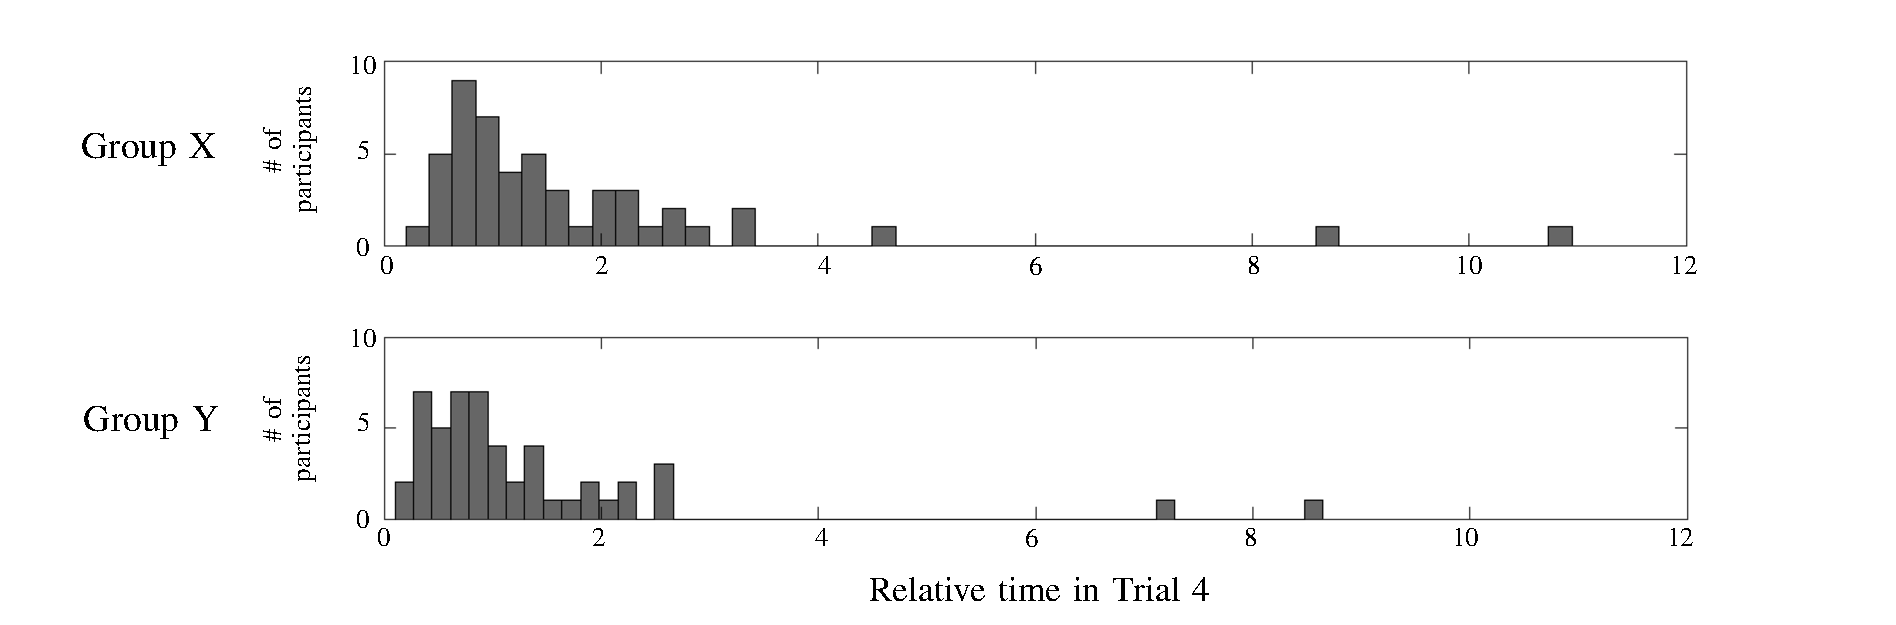
\includegraphics[scale=.5]{results_2.pdf}
\end{center}\caption{Relative time spent in Trial 4 by participants from the two groups, normalized by the time spent in Trial 5.}
\label{fig:results2}
\end{figure}



\subsection{Hypothesis \ref{Hip:FeatureBiasTimeAdvantage}}\label{Results:FeatureBiasTimeAdvantage} 
This hypothesis regarded the behavioral advantage of the feature stickiness effect, which we tested by comparing learning times in Trial 4 for participants of Groups X versus Y (see Figure~\ref{fig:results2}). If the feature stickiness bias represents a behavioral advantage, Group Y should learn concept $C^4_1$ faster than Group X. To avoid confounds due to inter-individual differences in absolute learning time, for this analysis we normalize individual learning times with the time spent in Trial 5, which uses different features than the previous concepts and should not be affected by any obvious inter-trial relation with previous concepts\footnote{indeed, Trial 5 was pre-registered as a `normalizer' trial}. The differences in the learning times between the groups are not significant if we analyze the data of all participants as shown in Figure~\ref{fig:results2} (two-sample t-test shows $t=1.26$,  $P=0.2$), but they are significant if we rule out from this analysis 5 outliers that spent more than 5 times in concept 4 than 5, or in concept 5 than 4 ($t=2.18$,  $P<0.05$) \footnote{The ANOVA proposed in the pre-registration also did not reveal significant differences in learning times. For simplicity in the analysis of the outliers, we replaced here the ANOVA for a simple t-test between the normalized learning times of the two groups.}
% We will also study the time spent in the learning phase (hypothesis (c)). Here, the category will be chosen such that only one of two groups will be able to show feature stickiness. In the third trial of the experiment, one of the groups will learn a concept that uses 2 variables (p1 and p2), and the other group will learn a concept with the same operators but with two other variables (p5 and p6). After this, both groups will learn the same category in the fourth trial, using p5 and p6. We will compare learning times between the two groups for the third and the fourth concept. To this end, we will perform a mixed ANOVA on the learning times with the concept trial as within-subject factor (trial 3 or 4) and the group as a between-subject factor (group A or B). We will test for the interaction between within- and between-subject factor. If the P-value of this ANOVA reveals that the interaction is significant, we will conclude that feature stickiness poses a significant advantage by reducing future learning times.


\subsection{Hypothesis \ref{Hip:StickinessFeatureOperator}} \label{Results:StickinessFeatureOperator} 
In this work we did not find conclusive evidence regarding this hypothesis. %, so we decided to leave it out of the results report. %(but see Section~\ref{sec:Discussion} for discussion).
 We suspect that the cause was an experimental setup that underestimated the strength of the bias favoring the $\AND$ operator over the $\OR$ operator. A future experiment could probe the existence of operator stickiness by having longer consecutive periods where feature reuse is not a useful bias and where only one logical operator remains useful for explaining a concept, before finally presenting a concept that can be explained via two different rules, each using different operators. Thus we leave for future work the task of studying the interaction between the feature stickiness bias and the precise structure of the logical rules being learnt. 



\subsection{MDL bias} \label{Resultados:MDLbias} 

The MDL-bias hypothesis posits that concept learning difficulty increases with its MDL \cite{feldman2000minimization}. %\sergio{\cite{feldman2003simplicity}?}
In addition to their other roles, Trials 3 (group X and Y), 4, and 5 served to test this hypothesis in the new framework of multiple consistent explanations. In these trials, there were two possible explanations that were consistent with the shown data, one of much higher MDL than the other (15 vs 3). For example, in the Group X of Trial~3, the short explanation was $p_1 \land p_2$, while the longer one was $((p_3 \lor (p_4 \lor p_5))\land(\lnot p_3 \lor ((p_4 \lor \lnot p_5)\land (p_5 \lor \lnot p_4))))$; the longer rule in other trials was always a substitution of features applied to this one (in order to keep the features disjoint between the two explanations). For these 3 trials, the responses of the $100$ participants add to a total of $300$ responses. From this total, $18$ responses in the generalization phase did not choose objects consistent with any of the two explanations; $2$ responses were consistent with the MDL 15 rule; and $280$ responses were consistent with the MDL 3 rule. While this expectation was somehow baked in the experimental design, we conclude that the MDL-bias hypothesis holds in this framework of multiple consistent explanations. Future work could explore in greater detail the relative difficulty of rules with slightly different MDL in this framework.


% When excluding individual responses of participants that did not choose a valid generalization in a trial ($N = 18$), we are left with a total of $282$ instances of a selection between the two explanations. \sergio{En el 4B no sé cómo interpretar el 0/39 para el MDL 15. Lo conté como 1 que es lo menos favorecedor.}
% In $280$ of these cases, the selection of the generalization set was consistent with a rule with MDL 3, while only $2$ were consistent with the MDL 15 rule.
% The probability of obtaining at most 2 cases selecting the longest rule under the null hypothesis of randomly choosing between the two explanations is $P<10^{-80}$.
% From this we conclude that the MDL-bias hypothesis holds in this framework of multiple consistent explanations. While this expectation was somehow baked-in the experimental design, we include this result as to more precisely and explicitly validate the assumption.


% \paragraph{Additional observations}\sergio{Posiblemente se puede sacar, editar, o mover a otro lado.}
% % Sergio: Estoy chamuyando, no sé qué se sabe del tema:
% However, it might be observed that this null hypothesis is very weak, given the natural expectation of longer rules being more difficult to learn. Let us consider the following alternative null hypothesis: ``In the presence of multiple explanations with different MDLs, let $S$ be the sum of all MDLs. Then the probability of a person selecting a particular explanation that corresponds to rule $\varphi$ equals $(S - MDL_\varphi) / S$''. In our case, the probability of the MDL 15 and MDL 3 rules would then be $3/18$ and $15/18$, respectively. Testing the observed data against this null hypothesis we obtain $P<10^{-20}$.


% We can even reject a more stringent null hypothesis, where the relative difficulty to find a longer solution doubles for every fixed increase in length of the rule. Thus, beginning from a probability of $0.5$ vs $0.5$ in the case of equal-length rules of MDL 3, we get that increasing the size of the first one 4 times by 3 leads to probabilities of $0.5 / 16 = 0.03125$ and $0.96875 = 1 - (0.5 / 16)$ respectively. Even in this case, we obtain that~$P<0.01$. %0.00663802183237036
% %\widesergio{Igual podría ser más estricta la Hip. null, si estuviesemos por ejemplo pensando cómo aumenta el espacio de posibles fórmulas con cada aumento en 1 de MDL. Supongo que de alguna manera es una hip. nula más neutra, que asume que la explicación se propone y chequea al azar tomada del espacio de todas las fórmulas posibles}


% \widesergio{Note (footnote en algún lado? borrar? pasar Future Work?: It seems reasonable to posit that additive increases in MDL result in multiplicative increases in difficulty. This would correspond in some manner to a weighted random sampling from the space of possible rules, giving more weight to smaller ones. However, the structure of the rule itself also seems to be of great importance, as we mention in~\S\ref{subsection:resultsPilot}; future works could explore how the rule structure and operators used affect the ease of finding new concepts.}



% \subsection{Hypothesis \ref{Hip:StickinessFeatureOperator}}

% This hypothesis was concerned with the existence and relative strength of stickiness effects related to features and to operators. By comparing the proportion of subjects that used the same features or the same logical operators between Trial~1 and Trial~2, we could detect a bias that strongly favors the reutilization of one of these characteristics over the other. 

% However, our analysis did not find any strong effect in favouring features stickiness over operator stickiness, nor viceversa.

% \widesergio{Pablo: Insertar datos}




%\widesergio{Posiblemente separar en los 4 subexperimentos. En cada subexperimento: para cada trial: rango de fallos antes de pasar a siguiente trial(+ mediana), rango de errores cuando hay fallos, rango de tiempo para completar con \'exito. Notar que no estamos incluyendo el rango de fallos ni de errores por fallo, pero lo reportamos por inter\'es que puedan hacer surgir (an\'alisis post hoc). Adem\'as, quiz\'as se podr\'ia considerar individualmente la diferencia proporcional de tiempo entre los trials y luego poner los rangos generales de estos valores}

%\subsection{Choice of generalization examples and verbal explanations}
%\widesergio{Hice esta secci\'on ac\'a, pero puede ser que corresponda en  Discussion o en otro lado}
%Most of the time, participants in the generalization stage gave a verbal explanation that was consistent with a positive description of a category, as was expected in the experiment design. However, there were some instances of negative descriptions, such as those of the type `boxes with these kind of elements do not belong to the category'. These two types of internal representation could potentially affect results for Hypothesis~\ref{Hip:AndOverOr} and Hypothesis~\ref{Hip:StickinessFeatureOperator}, since the testing of those hypotheses depends on distinguishing the utilization of operators in a context where the exact rule used cannot be inferred solely from the choice of generalization examples (since e.g. `$A\land B$' is logically equivalent to `$\lnot(\lnot A\lor \lnot B)$'). 

%Regarding Hypothesis~\ref{Hip:AndOverOr}, \sergio{Habr\'ia que volver a analizar los resultados mirando las explicaciones verbales de estas personas en el Trial 1 cambia algo (seguramente queda m\'as grande el p). Ver comments para lista. Ver .txt en Dropbox}

% Lista donde solo aparece una descripcion que puede ser problematica para analisis
% [1, "ExplicacionCategoria", "Elements that do not have both a down arrow and the letter B."]
% [1, "ExplicacionCategoria", "Boxes are disqualified if they have either the letter B or a moon."]
% [1, "ExplicacionCategoria", "if the heart symbol present in any of the box then the box does not belong to the category. the same as follows if the number 9 present it didn't belong to the category"]
% [1, "ExplicacionCategoria", "does not include B and sun together"]
% [1, "ExplicacionCategoria", "Down arrows and exclamation points or up arrows and exclamation do not belong to the category."] %No parece completa esta descripcion
% [1, "ExplicacionCategoria", "Anything that doesn't include the exclamation and/or triangle belong to category."]
% [1, "ExplicacionCategoria", "Items that do NOT contain BOTH a 9 and a play button symbol belong to the category."]
% [1, "ExplicacionCategoria", "The elements: turquoise right pointing triangle and downward pointing red arrow are not to be found in boxes qualifying as belonging to the category. Therefore any box containing either or both of those elements do NOT belong to the category. All the other elements may or may not be used in boxes, and may be used in any order or position."] 
%[1, "ExplicacionCategoria", "Apparently if doesn't have a B and a right arrow it belongs to the category"]
% Despues quizas hay un par mas que son ambiguos.

% The results for Hypothesis~\ref{Hip:StickinessFeatureOperator} were inconclusive, but future attempts to revisit the question should remember to take care in accounting for the possibility of misinterpreting the results if the verbal explanations are excluded from the analysis. PABLO: esto ya lo mencione antes, no hace falta volverlo a poner.

%%%%%%%%%%%%%%%%%%%%%%%% DISCUSSION %%%%%%%%%%%%%%%%%%%%%%%%%%%%

%!TEX root = Main.tex

\section{Discussion}\label{sec:Discussion}


We designed an experimental framework in which participants observe an incomplete set of examples, which are consistent with two alternative minimal descriptions depending on which features are observed.  We illustrated several advantages of our method compared to separately presenting sets of examples consistent with only one minimal description at a time. First, we showed that when a set of examples is consistent with a disjunction \textit{and also} with a conjunction, participants are more likely to find the conjunction, in accordance with well-known previous results that show that the conjunction is learnt faster than the disjunction when presented separately \cite{bourne1970knowing}. Then, we showed that when rules of significantly different MDL are consistent with the observations, almost all participants discover the simpler rules, consistent with previous result showing that, when rules of different MDL are tested separately, learning times are proportional to MDLs \cite{feldman2000minimization}. Finally, we showed that when the logical structure of the minimal rules is independent of the selected features, participants are more likely to reuse the same features used to describe previous concepts, which allows them to learn concepts faster than a control group that is not reusing features. To our knowledge this effect has not been previously characterized in the concept-learning literature, adding to the library of effects illustrating how human attention is biased towards features that are useful to describe the concepts (see \cite{blair2009extremely,kruschke2000blocking,kruschke2005eye,hoffman2010costs}, among others).
\color{black}
% We first showed in \S\ref{Results:AndOverOr} that feature attention depends on the form of the minimal description using those features (e.g. conjunction vs. disjunction), as well as on the relative MDL of the two minimal descriptions (participants used the features that lead to a shorter minimal description, \S\ref{Resultados:MDLbias}). We then showed with  \S\ref{Results:FeatureBiasStickiness} and \S\ref{Results:FeatureBiasTimeAdvantage} that if the minimal description is the same independently of the chosen features, participants are more likely to reuse the same features used to describe previous concepts, which allows them to learn concepts faster than a control group that is not reusing features.

Eye-tracking studies in categorization tasks have revealed that feature attention rapidly changes between trials depending on which features are relevant for classification in each trial~\cite{blair2009extremely}, as well as depending on prior knowledge about feature relevance \cite{kim2011prior}.  

In \cite{kruschke2005eye} it is found that eye movements confirmed that attention was learned in the basic learned inhibition paradigm, and in \cite{hoffman2010costs} it is also found that eye movements revealed how an attention profile learned during a first phase of learning affected a second phase. \color{black} Our experimental setup allows us to test an arguably simpler complementary hypothesis: everything else being equal, participants are biased to use the same features used in the past.  Importantly, we were only able to test this hypothesis thanks to our framework, which allows us to present a set of examples consistent with two rules of exactly the same logical structure, but using different sets of features. Then, without using eye-tracking, we can recover which rule the participants learned, and thus which set of features they attended to. Since the two sets of features explain the examples using exactly the same logical structure, preferentially explaining the concept using one set of features over the other can only be due to a preference over the features themselves, and not a preference over alternative logical structures. 

% Rather than being a superficial nuisance in concept learning, the feature stickiness bias may have important computational consequences: in environments where concept complexity depends on which features are used to describe them, the feature stickiness bias allows for less complex representations \cite{bengio2013representation,lake2015human}, maximizing the expected value of future computations within resource-bounded constraints \cite{gershman2015computational}. 
\color{black}



Although some of the hypothesis that we test are aligned with the well-known Einstellung effect \cite{luchins1942mechanization} which states that adopted solutions may hinder simpler ones when aiming at tackling novel problems, our experimental setting is different to the classical water jar test 
\color{blue}
(the most commonly cited example of an Einstellung effect, where participants need to discover how to measure a certain amount of water using three jars with different and fixed capacity)
\color{black}
in two senses. First, we do not drive the experiment to control and supervise the aspects that participants have to pay attention to. On the contrary, our focus is on the {\em choice} of the features that show to be useful for learning a concept with more than one rational explanation. Second, our experimental framework goes along the \color{blue} Language of Thought (LoT) hypothesis \cite{fodor1975language}, which states that the human capacity to describe concepts -—and, more generally, of all elements of thought—- builds on the use of a symbolic and combinatorial mental language
\color{black}
and it is specifically conceived to handle expressions in propositional Logic (but expansible to other formal languages), which is the ground where the rational explanations can be formalized. Such approach enables us to treat the notion of {\em feature} in a very precise way. Another well-studied phenomenon related to our work is Kamin’s cue {\em blocking}, where the learning of a given stimulus B is {\em blocked} by the mere fact that it was preceded by a set of stimuli A that already pairs with the outcome. This shows that the subject learned that stimulus B was not useful, and hence disregards their attention to it in the upcoming events \cite{wagner1970stimulus,mackintosh1975theory,rescorlaw72}. Studied in humans in \cite{chapman1990cue, arcediano1997blocking, kruschke2000blocking} among others, our work differs from these approaches in that we never introduce a stage were a feature A is intentionally exposed in absence to B, in order to guide the attention of the participant. %Instead, in our setting the set of features the participants are exposed to is constant during each test.  %\sergio{En realidad sacamos 2 y ponemos dos para Trials 5 y 6}
\color{black}


% Categorization? o Category learning?
% In addition, the controlled logical setting used in our experiment shows that when observing an incomplete set of examples, as is almost always the case in the real world, the concept learning biases that have been previously studied \cite{ashby2011human} are a principal determinant of the features used to describe the concept. We showed this in particular for the conjunction-disjunction bias \cite{bourne1970knowing} and the MDL bias \cite{feldman2000minimization}. Thus our experiment illustrates a powerful metalearning property of the seemingly simple feature stickiness bias. If \textit{(1)} the subjective complexity of concept descriptions is correlated with the features used to describe them, and \textit{(2)} participants are more likely to describe concepts using features that lead to simpler explanations (as we showed in our experiment), then the feature stickiness bias minimizes the expected complexity of concept descriptions. 

% In this work, we focus only on transfer learning effects based on the features chosen to describe concepts. We acknowledge, however, that several other transfer learning effects are present in human sequential logical concept learning, such as when subsequent concepts differ in their hierarchical structure \cite{tano2020towards}, when changing the relevant features in subsequent exclusive disjunctions \cite{kruschke1996dimensional}, or when two concepts are learned in an interleaved or a focused manner
% ~\cite{carvalho2014putting}. Similarly to the transfer learning hierarchical structure bias \cite{tano2020towards}, our work demonstrates that rather than being a superficial nuisance in concept learning, the feature stickiness bias may have important computational consequences: in environments where concept complexity depends on which features are used to describe them, the feature stickiness bias allows for less complex representations \cite{bengio2013representation,lake2015human}, maximizing the expected value of future computations within resource-bounded constraints \cite{gershman2015computational}. 

% Another major contribution of this work is the experimental setup (as schematically shown in Figure~\ref{fig:trials}). Although we use it mainly to characterize the feature stickiness bias, it constitutes a general framework to study concept learning biases. 

We conjecture that most first-order determinants of subjective concept difficulty will also hold in a relative manner in our dual-concept setup, such as the MDL bias (for less extreme cases than evaluated in this work) \cite{feldman2003simplicity} and the transfer learning hierarchical structure bias \cite{tano2020towards}. Importantly, our experimental setup also allows to directly test second-order subjective difficulty effects (e.g.\ concept A is learnt faster if presented jointly with concept B than with concept C), as well as second-order transfer learning effects (e.g.\  participants learn more rapidly concept C if they have first observed concept A coupled with B$_1$, compared to A coupled with B$_2$). We believe that a systematic study of concept learning difficulty with two (or more) concepts presented at the same time in each trial may open a new window into the dynamics of human concept-learning mechanisms. For example, consider the study in \cite{piantadosi2016logical}, where participants gradually learn one concept while simultaneously selecting elements currently believed to belong to that concept. Here, the authors fit a Bayesian language model to participants' choices in order to illustrate how the posterior probability of the different rules in the grammar varied across time, to approximate the order in which different rules are learned. In contrast, using our experimental setting we can directly estimate, in a model-free manner, the probability that each rule is learnt faster than another. One simply needs to jointly present (in an incomplete and mutually compatible way) a set of examples consistent with those two minimal rules, and then measure the fraction of participants that discover each rule.

Usually, concept learning biases have been studied in an isolated manner: the participant observes examples indicated as inside or outside a \textit{single} concept, and the experimenter evaluates its subjective difficulty for the participant. Although different methods have been used to present the concept to the participant (e.g.\ all elements at the same time \cite{tano2020towards,kemp2012exploring} or small sets of elements presented in series \cite{piantadosi2016logical}), to the best of our knowledge all previous category-learning studies have attempted to evaluate a single concept at a time. Here, we present a controlled logical setting to evaluate the relative difficulty of two concepts presented at the same time and under the same experimental conditions, and the framework could be generalized to more concepts straightforwardly. 

%/pablo{Mande el parrafo de operator stickiness a Experiment.}

%\widesergio{Quizás conviene terminar de una manera más fuerte, recalcando las posibilidades abiertas por el experimental setup nuevo. Hay una sección de Conclusions en BRM?}
%\widesanti{no veo que haya un template de secciones}

% \input{future}

\paragraph{Open Practices Statement.} This study's methodology, data collection procedures, sample size, exclusion criteria, and hypotheses were preregistered on the Open Science Framework (OSF) in advance of the data collection and analysis, in order to ensure transparency, reproducibility, and rigour. The preregistration of this study can be found at \url{https://osf.io/mgex3}. The actual experiment, together with all the experimental data analyzed, is available online at \url{https://osf.io/gtuwp/}.